\documentclass[10pt]{book}


\title{Introduction to Fluid Dynamics}
\author{Joseph D. MacMillan}
\date{\vspace{2in} \small This work is licensed under a \href{https://creativecommons.org/licenses/by-sa/4.0/}{Creative Commons Attribution-ShareAlike 4.0 International License}. \\ \vspace{0.5in} This version of the book was created on \today. You can always find the most up-to-date version at {\footnotesize \url{https://faculty.uoit.ca/macmillan/IntroFluidDynamics} (web)} or \\ {\footnotesize \url{https://faculty.uoit.ca/macmillan/IntroFluidDynamics/IntroFluidDynamics.pdf} (PDF)}.}

\usepackage[a5paper]{geometry}

\usepackage{graphicx}
\usepackage{color} 

\usepackage{amsmath, amssymb}

\usepackage[T1]{fontenc}
\usepackage{libertine}
\usepackage[libertine]{newtxmath}

\newcommand{\uu}{\mathbf{u}}
\newcommand{\grad}{\boldsymbol{\nabla}}
\renewcommand{\div}{\boldsymbol{\nabla} \cdot}
\newcommand{\curl}{\boldsymbol{\nabla} \times}
\newcommand{\dfdx}[2]{\frac{\partial {#1}}{\partial {#2}}}
\newcommand{\ddfdx}[2]{\frac{\partial^2 {#1}}{\partial {#2}^2}}
\newcommand{\vort}{\boldsymbol{\omega}}

\newcounter{example}[chapter]
\def\theexample{\thechapter.\arabic{example}}
\newenvironment{example}[1][ ]{\refstepcounter{example}
\noindent
\nopagebreak
\vspace{5pt}
\nopagebreak
\hrule
\nopagebreak
\vspace{5pt}
\nopagebreak
\textbf{Example \theexample \ -- #1.}
\nopagebreak

\noindent \leftskip4em
}
{ 
%\noindent \rule{\textwidth}{.4pt}
\vspace{5pt}
\hrule
\vspace{5pt}
}

\newcounter{problem}[chapter]
\def\theproblem{\thechapter.\arabic{problem}}
\newenvironment{problem}[1][ ]{\refstepcounter{problem} \noindent \textbf{Problem \theproblem \ -- #1.}}{\vspace{0.1in}}

\usepackage[hang, small, bf]{caption}
\captionsetup[table]{position=top}
\captionsetup[figure]{position=bottom}

%\usepackage[toc, page]{appendix}

%\usepackage{listings}

\usepackage[hidelinks]{hyperref}
\hypersetup{pdftitle={Introduction to Fluid Dynamics}}
\hypersetup{pdfauthor={Joseph D. MacMillan}}
\urlstyle{rm}

\begin{document}

\maketitle

\tableofcontents

\chapter{Introduction}

\section{Opening Thoughts}

What, exactly, is a fluid? Well, it's anything that \emph{flows}, of course. But that can mean a surprising number of things.

One obvious example is water, which we'll use extensively as our go-to fluid for a number of applications. Other fluids might be highly viscous -- syrup is a good example -- in which case the behaviour might be very different.  Later on in the book we'll take an introductory look at \emph{aerodynamics}, where the fluid is of course air.  

These are all good examples of what's called a \emph{Newtonian fluid} -- the fluid has certain, fairly simple properties and can be modelled well by a set of equations called the \emph{Navier-Stokes} equations.  Other fluids, though, are more complicated (and, for the most part, beyond the scope of this book).

For example, the behaviour of fluids with a net charge (e.g., a plasma) add interesting complications that must be dealt with by including the theory of electricity and magnetism.  Combining Maxwell's equations with the Navier-Stokes equations leads to the theory of magnetohydrodynamics, or MHD for short.

Even something as commonplace as blood, though, can be beyond the Navier-Stokes equations to model.  That's because blood is an example of a non-Newtonian fluid -- it's nonhomogeneous and is a ``shear-thinning'' fluid, which means it becomes less viscous at high shear strain.  Consider what happens to the blood during an anaphylactic shock -- an extreme allergic reaction.  The body's first response is to release histamine, which causes the blood vessels to widen.  When this happens, the blood will slow down, for reasons we'll learn have to do with conservation of mass.  But because blood is shear-thinning, it becomes more viscous as it goes slower.  This leads to a feedback loop -- increased viscosity causes the blood to slow further, causing it to be more viscous, which means the blood slows even more, and so on.  This is why anaphylaxis is so severe and needs to be treated right away with adrenaline, which increases blood flow.

As a final, surprising, example, traffic can sometimes be modelled as a fluid -- even though cars are large, discrete objects.

Although the study of fluid dynamics is centered around solving the Navier-Stokes equations, in this first chapter we'll begin with some preliminary ideas about the flow of fluids, in particular how we can mathematically describe and visualize it.  But before we start with the heavy lifting of solving differential equation, we'll also need to be able to identify various properties of the fluid, such as its vorticity and viscosity, since in many cases understanding these can lead to significantly simpler methods of solving the equations of fluid dynamics.



\section{Describing Fluid Flow}

The main goal of fluid dynamics is to find the fluid velocity $\bf{u}$ at every point $\bf{x}$ at any time $t$:
\begin{equation}
\mathbf{u} = \mathbf{u}(\mathbf{x}, t).
\end{equation}
This is a good time to discuss some of the notation we'll be using.  First, note that I'm bolding any quantity that's a \emph{vector}, like position and velocity.  Scalars are represented by italicized letters.  Secondly, I'm using $\mathbf{u}$ to denote the velocity rather than the more usual $\bf{v}$. In fact, the letter $v$ serves a different purpose -- it's the $y$ component of the fluid velocity. The $x$ and $z$ components are denoted by $u$ and $w$, respectively, so we can write the full vector form of the velocity as
\begin{equation}
\mathbf{u} = u \, \hat{i} + v \, \hat{j} + w \, \hat{k} = [u, v, w].
\end{equation}
Keep in mind that $u$, $v$, and $w$ are each functions of $x$, $y$, $z$, and time:
\[
u = u(x, y, z, t), \quad v = v(x, y, z, t), \quad \text{and} \quad w = w(x, y, z, t),
\]
and note that I'm using some vector short hand with the square brackets.

This can sometimes be confusing notation, so be careful with it.  Also note that (to add to the confusion) $u$ does double duty: it's both the $x$ component of the flow, as well as the name of the entire velocity vector field.


\begin{figure}
\centering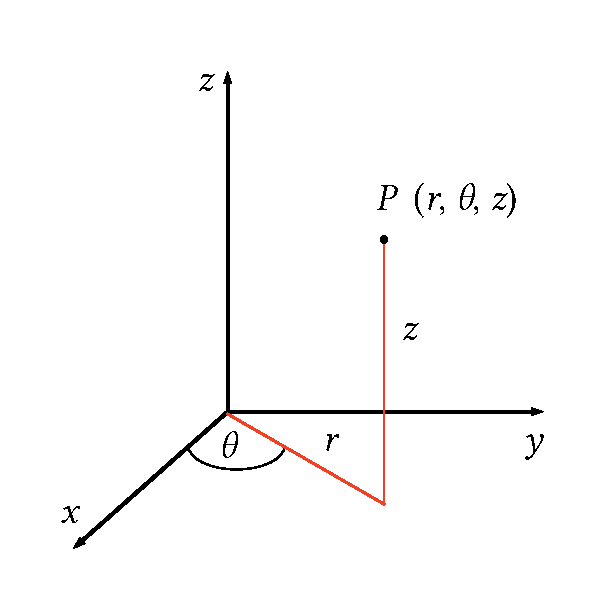
\includegraphics[width=0.5\linewidth]{Figures/Chapter1/fig_cyl_coord}
\caption{Cylindrical coordinates $(r, \theta, z)$.}
\label{fig_cyl_coord}
\end{figure}

So far, I've written everything down in Cartesian coordinates, but we'll use cylindrical coordinates $(r, \theta, z)$ frequently as well.  Figure \ref{fig_cyl_coord} shows the usual cylindrical coordinate setup (note that I'm using $\theta$ rather than the usual $\phi$; this is mostly because all my notes come from a math book), and it's clear that
\[
x = r \cos \theta, \quad y = r \sin \theta, \quad \text{and} \quad z = z.
\]
We can write the fluid velocity in cylindrical coordinates as
\begin{equation}
\label{eq_u_cyl}
\mathbf{u} = u_r(r, \theta, z, t) \hat{r} + u_\theta (r, \theta, z, t) \hat{\theta} + u_z(r, \theta, z, t) \hat{z}.
\end{equation}
I'll avoid using the ``bracket'' shorthand if we're using cylindrical coordinates, though.



In much of our examination of fluid dynamics, we'll deal with special cases and symmetries which will make our job (slightly) easier.  The below examples discuss two of these special cases.

\begin{example}[Steady Flow]
A \emph{steady flow} has no explicit time dependence, so that
\begin{equation}
\frac{\partial \mathbf{u}}{\partial t} = 0.
\end{equation}
This means that, at any point, the speed and direction of the flow are constant. We'll be dealing with this case quite frequently, especially at the beginning of the book.
\end{example}

\begin{example}[Two Dimensional Flow]
A \emph{two dimensional} flow has the form
\begin{equation}
\mathbf{u} = [u(x, y, t), v(x, y, t), 0].
\end{equation}
Note that not only is there no $z$ component to the velocity field, but there is furthermore no $z$ dependence on the
$x$ and $y$ components, either.
\end{example}





\section{Visualizing Fluid Flow}



\subsection{Vector Plots}

One way to visualize the flow of a fluid is by drawing a vector for $\mathbf{u}$ at a sample of positions and, if necessary, times.

\begin{example}[Flow about a stagnation point]
For example, consider the fluid velocity vector field
\begin{equation}
\label{eq_stag}
\mathbf{u} = [\alpha x, -\alpha y, 0].
\end{equation}
This is an example of two-dimensional, steady flow, and, as we'll see later, is the flow around a \emph{stagnation point}, which is a point in the fluid which is not flowing.  The vector plot for this flow is given in Figure \ref{fig_vector_plot}. 
\end{example}

\begin{figure}
\centering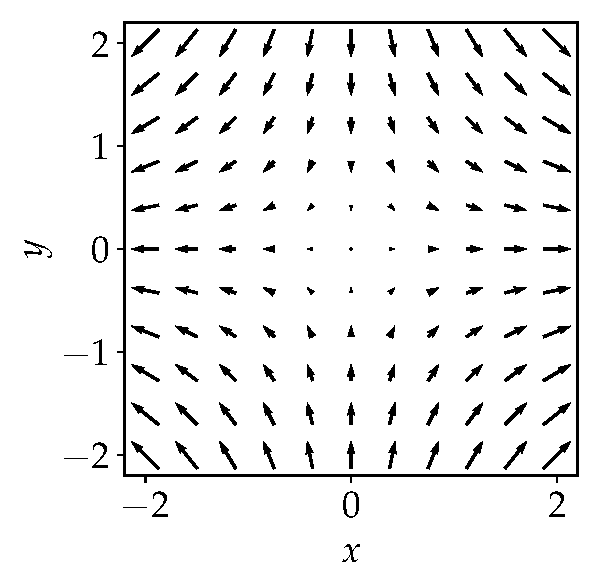
\includegraphics[width=0.5\linewidth]{Figures/Chapter1/fig_vector_plot}
\caption{A vector plot for flow about a stagnation point.  Here the parameter $\alpha = 1$.  Note that at the point $(0,0)$ the flow velocity is zero; that's what makes it a stagnation point. \href{[Link to Code]}
\label{fig_vector_plot}
\end{figure}



\subsection{Streamlines}

A more common way to visualize fluids is with \emph{streamlines}.  A streamline is a curve that, at time \(t\), has the same direction as \(\mathbf{u}(\mathbf{x}, t)\) at each point. This is a concept you might be familiar with from electrodynamics -- electric field lines are very similar.  Like field lines, streamlines can't cross, since that would imply that a particular fluid element at that point would have two different velocities.  

How do we calculate (and plot) streamlines? Well, we first parameterize a streamline curve, using \(s\) as the parameter, as 
\[
x(s), \quad y(s), \quad z(s),
\] 
so that, as \(s\) changes, the functions $x$, $y$, and $z$ trace out the streamline curve.   From the definition of a streamline, we know that
\[
\frac{dx}{ds} = ku, \quad \frac{dy}{ds} = kv, \quad \frac{dz}{ds} = kw,
\] 
where \(k\) is some constant (and different streamlines will have different -- but unique -- values of \(k\)). Since \(k\) is the same along each streamline, we must have
\begin{equation}
\frac{dx/ds}{u} = \frac{dy/ds}{v} = \frac{dz/ds}{w}.
\end{equation} 
This means that, given the functional form of \(u\), \(v\), and
\(w\), we can find \(x(s)\), \(y(s)\), and \(z(s)\).

In addition to streamlines, \emph{pathlines} and \emph{streaklines} are sometimes used to visualize and describe fluid flow.  However, for steady flow -- which we'll mostly be dealing with -- they're the same as streamlines, so we won't worry about them too much.  You can watch a nice video about it (as well as some other aspects of visualizing fluids) at \url{https://youtu.be/nuQyKGuXJOs}\footnote{This is just one video in a whole series by the National Committee for Fluid Mechanics Films.  Despite their age, they're great, and I highly recommend watching the ones that are relevant to us.}, and Problem \ref{prob_unsteady} takes a look at an unsteady case where the path lines are different from the streamlines.

\begin{example}[Plotting Streamlines]
As an example of calculating and then plotting streamlines, let's go back to our flow about a stagnation point, Equation \ref{eq_stag}.  Since this is two dimensional flow, we can ignore $w$ and $z$ dependence and look at 
\[
\frac{dx/ds}{u} = \frac{dy/ds}{v}.
\]
Plugging in \(u\) and \(v\) for this case, and removing the parameter $s$ for simplicity, gives us
\[
\frac{dx}{\alpha x} = -\frac{dy}{\alpha y}.
\] 
Integrating both sides and solving for \(y\) gives the function 
\begin{equation}
y(x) = \frac{c}{x}.
\label{eq_stream_ex}
\end{equation}
That's our answer; \(c\) is the integration constant, which will vary from streamline to streamline.  Figure \ref{fig_streamline_example} shows the streamlines plotted; as usual, code to do this is provided separately.
\end{example}

\begin{figure}[t]
\centering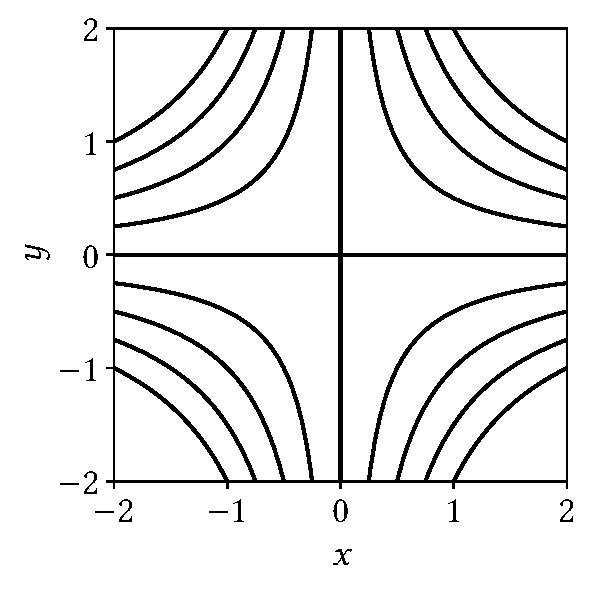
\includegraphics[width=0.5\linewidth]{Figures/Chapter1/fig_streamline_example}
\caption{Streamlines plotted from Equation \ref{eq_stream_ex}, for a variety of values of $c$ ranging from $-2$ to $2$.  Note that the streamlines cross at the stagnation point; that's the only place where they're allowed to.}
\label{fig_streamline_example}
\end{figure}







\section{Total Derivative and Acceleration}

Now that we know how to visualize the flow of a fluid, we need to be able to calculate how it \emph{changes}.  

Let $f(x, y, z, t)$ be some quantity of interest -- it might be a component of velocity ($u$ or $v$, say), or maybe the density of the fluid $\rho$, or even the concentration $c$ of a certain pollutant in the fluid.  If we're then looking at one particular (fixed) location -- say, $x, y, z$ -- in the fluid, then $\partial f / \partial t$ gives the rate of change of $f$ at that position.

On the other hand, we might want to know how $f$ changes as we move along with the fluid.  In this case, we might imagine attaching ourselves to a certain \emph{fluid element} -- a small ``blob'' of the fluid -- and measuring how $f$ changes as we move along with it.  This rate of change is given by the so-called \emph{total} or \emph{material} derivative,\footnote{There are many other names for this kind of derivative, too; according to Wolfram MathWorld, it's also called the convective derivative, the advective derivative, derivative following the motion, hydrodynamic derivative, and Lagrangian derivative, among a few others.}
\[
\frac{Df}{Dt} \equiv \frac{df}{dt} = \frac{d}{dt} f[x(t), y(t), z(t), t].
\]
Now, $x(t)$, $y(t)$, and $z(t)$ all change as we move with the flow, and of course
\[
\frac{dx}{dt} = u, \quad \frac{dy}{dt} = v, \quad \text{and} \quad \frac{dz}{dt} = w.
\]
So, applying the chain rule to the derivative above, we get
\begin{align*}
\frac{Df}{Dt} & =  \frac{\partial f}{\partial x}\frac{dx}{dt} + \frac{\partial f}{\partial y}\frac{dy}{dt} + \frac{\partial f}{\partial z}\frac{dz}{dt} + \frac{\partial f}{\partial t} \\
& = u \frac{\partial f}{\partial x} + v \frac{\partial f}{\partial y} + w \frac{\partial f}{\partial z} + \frac{\partial f}{\partial t}.
\end{align*}
This can be written more compactly using vectors:
\begin{equation}
\label{eq_total_deriv}
\boxed{
\frac{Df}{Dt} = \frac{\partial f}{\partial t} + (\mathbf{u} \cdot \boldsymbol{\nabla}) f.
}
\end{equation}
Careful with that dot product; the gradient operator $\boldsymbol{\nabla}$ operates on the function $f$, so you can't switch the order.  In this case, $(\mathbf{u} \cdot \boldsymbol{\nabla}) \neq (\boldsymbol{\nabla} \cdot \mathbf{u})$.

As an example of applying the total derivative, let's take $f$ to be the fluid velocity itself:
\begin{equation}
\label{eq_accel}
\boxed{
\frac{D\mathbf{u}}{Dt} = \frac{\partial \mathbf{u}}{\partial t} + (\mathbf{u} \cdot \boldsymbol{\nabla}) \mathbf{u}.
}
\end{equation}
This, as you might suspect, is the \emph{acceleration} of the fluid element at position $\mathbf{x}$.

Note that if the material derivative is \emph{zero},
\[
\frac{Df}{Dt} = 0,
\]
that implies that the quantity $f$ doesn't change \emph{for a particular fluid element.}  On the other hand, if just
\[
(\mathbf{u} \cdot \boldsymbol{\nabla}) f = 0,
\]
that means that $f$ will be constant \emph{along a streamline.}  This isn't obvious (at least to me), so let's prove it.  Let $\hat{\mathbf{e}}_s$ be a unit vector that is always parallel to a streamline in the direction of the flow.  Since a streamline is always tangent to the flow, we can write
\[
\mathbf{u} = |\mathbf{u}| \, \hat{\mathbf{e}}_s,
\]
so that
\[
(\mathbf{u} \cdot \boldsymbol{\nabla}) f = (|\mathbf{u}| \, \hat{\mathbf{e}}_s \cdot \boldsymbol{\nabla}) f = (|\mathbf{u}| \frac{\partial }{\partial s} )f = |\mathbf{u}| \frac{\partial f}{\partial s} = 0.
\]
Thus $\partial f / \partial s = 0$ and the quantity $f$ must be constant along the direction $s$, which is along the streamline.

\begin{example}[Acceleration of the fluid]
Let's return to our flow around a stagnation point.  What is the acceleration of the flow?

Well, clearly $\partial \mathbf{u} /\partial t = 0$ (the flow is steady), and so
\[
\frac{D \mathbf{u}}{Dt} = (\mathbf{u} \cdot \boldsymbol{\nabla} ) \mathbf{u} = \left( u \frac{\partial}{\partial x} + v\frac{\partial}{\partial y} \right) \mathbf{u}.
\]
At this point is probably easiest to work out each vector component separately:
\[
\frac{D u}{Dt} =  u \frac{\partial u}{\partial x} + v\frac{\partial u}{\partial y}  = \alpha^2 x,
\]
and
\[
\frac{D v}{Dt} =  u \frac{\partial v}{\partial x} + v\frac{\partial v}{\partial y}  = \alpha^2 y.
\]
So the acceleration is
\[
\frac{D \mathbf{u}}{Dt} = \alpha^2 x \, \hat{i} + \alpha^2 y \, \hat{j} = [\alpha^2 x, \alpha^2 y].
\]

\end{example}




\section{Incompressible and Irrotational Flow}

\subsection{The Incompressibility Condition}
\label{sec_incompressibility}

Except in one notable case -- gas dynamics -- we'll be dealing with fluids that are \emph{incompressible}.  This essentially just means that the density of the fluid is constant under pressure -- you can't compress it; stated another way, it means that a ``dyed'' blob of fluid can't change in volume as it moves.  Water is a good example of an incompressible fluid, and we'll even treat air as incompressible in some cases.

We need to be able to write down a mathematical statement of incompressibility.  To do this, consider a fixed, closed surface $S$ in the fluid.  By ``fixed,'' I mean that it's fixed in space, so fluid can move into this closed volume $V$ at some places and out at others; if the fluid is incompressible, though, then however much fluid is \emph{entering} the region must equal the amount that is \emph{leaving}.  

\begin{figure}
\centering
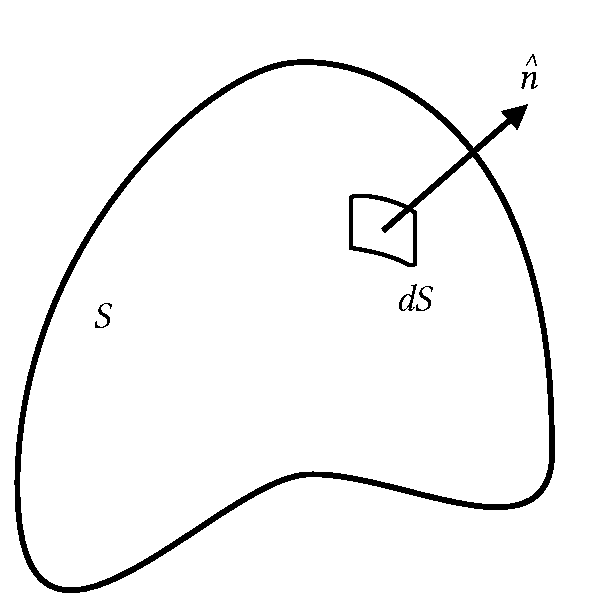
\includegraphics[width=0.5\linewidth]{Figures/Chapter1/fig_closed_surface}
\caption{A fixed, close surface.}
\label{fig_closed_surface}
\end{figure}

Consider, then, an infinitesimally small piece of $S$ -- call it $dS$ (see Figure \ref{fig_closed_surface}).  The amount of fluid that is leaving $V$ through $dS$ is given by
\[
\mathbf{u} \cdot \hat{n} \, dS.
\]
This expression, where $\mathbf{u}$ is the fluid velocity at the location of $dS$ and $\hat{n}$ points normal to the surface $dS$ but in the outward direction, is a \emph{volume flow rate}.  It measures the volume of fluid that passes through $dS$ per unit time.  The dot product ensureS we get only that fluid which is moving \emph{through} the tiny surface, whether it's flowing outward (positive dot product) or inward (negative dot product).

To find the total amount of fluid leaving the entire surface $S$, we can just integrate over that surface:
\[
\int_S \mathbf{u} \cdot \hat{n} \, dS
\]
is the net volume rate at which fluid is leaving.  However, for an incompressible fluid, we know this must be \emph{zero}.

To write this in a form a little more usable, we can apply the divergence theorem (you remember that from vector calculus, right?),
\[
\int_S \mathbf{F} \cdot \hat{n} \, dS = \int_V \boldsymbol{\nabla} \cdot \mathbf{F} \, dV,
\]
where $\mathbf{F}$ is some general vector field.  Our incompressibility condition then becomes
\[
\int_V \boldsymbol{\nabla} \cdot \mathbf{u} \, dV = 0.
\]
However, this must be true \emph{anywhere} in the fluid and for any size volume; that means the integrand itself must be zero:
\begin{equation}
\label{eq_incompressibility}
\boxed{
\boldsymbol{\nabla} \cdot \mathbf{u} = 0.
}
\end{equation}
This is the \emph{incompressibility condition}; unless we say otherwise, every flow must obey it.

\begin{example}[Incompressible flow]
Is our flow about a stagnation point incompressible?  Let's check.  Recall that $\uu = [\alpha x, -\alpha y]$.  The divergence of $\mathbf{u}$ is then
\[
\div \uu = \frac{\partial u}{\partial x} + \frac{\partial v}{\partial y} = \alpha + (-\alpha) = 0,
\]
just as we require.
\end{example}


\subsection{Vorticity}

The \emph{vorticity} of a flow is defined as
\begin{equation}
\boldsymbol{\omega} = \boldsymbol{\nabla} \times \mathbf{u}.
\end{equation}
For a two dimensional flow $\uu = [u(x, y), v(x, y), 0]$, we can write the vorticity as $\boldsymbol{\omega} = [0,0,\omega]$, where
\[
\omega = \frac{\partial v}{\partial x} - \frac{\partial u}{\partial y}
\]
(note the difference between the bolded $\boldsymbol{\omega}$ and the non-bold $\omega$ -- one is the full vector, and one is just the magnitude of that vector).

What, exactly, is vorticity?  It's related to the \emph{rotation} of the flow, but is a little trickier than that.  A couple of examples is probably best first.

\begin{example}[Vorticity of shear flow]
The flow given by $\uu = [\beta y, 0, 0]$ is called a \emph{shear flow}; a vector plot is shown in Figure \ref{fig_shear}.  This fluid is clearly \emph{not} rotating, but it does have vorticity.  Since it's two dimensional, we can easily calculate $\omega$:
\[
\omega = \frac{\partial v}{\partial x} - \frac{\partial u}{\partial y} = -\beta.
\]
\end{example}

\begin{figure}
\centering
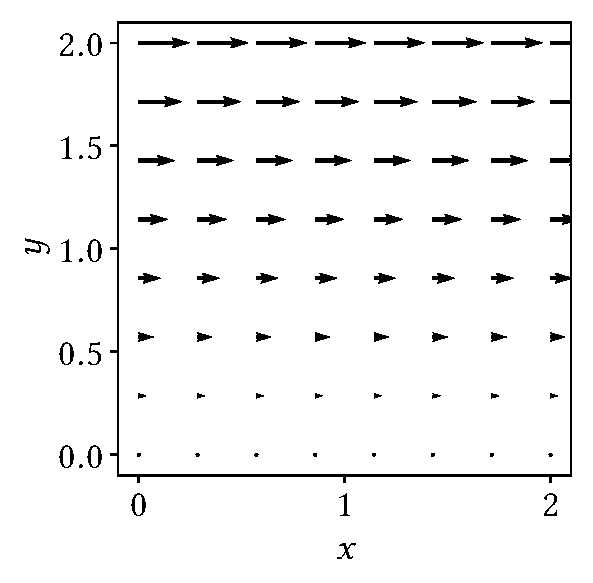
\includegraphics[width=0.5\linewidth]{Figures/Chapter1/fig_shear_vector}
\caption{A shear flow, with $\beta = 1$.}
\label{fig_shear}
\end{figure}

\begin{example}[Vorticity of line vortex]
\label{ex_vorticity_line_vortex}
Next, let's look at the flow
\begin{equation}
\uu = \frac{k}{r} \, \hat{\theta}.
\end{equation}
This is written in cylindrical coordinates, and the vector plot is shown in Figure \ref{fig_vortex}.  We'll be seeing this kind of flow quite a bit, so make sure you're familiar with it -- but for now all we need to know is that the fluid is clearly rotating.  Despite this, the vorticity is actually zero; I'll let you show this for homework (see Problem \ref{prob_vortex_vorticity}).
\end{example}

\begin{figure}
\centering
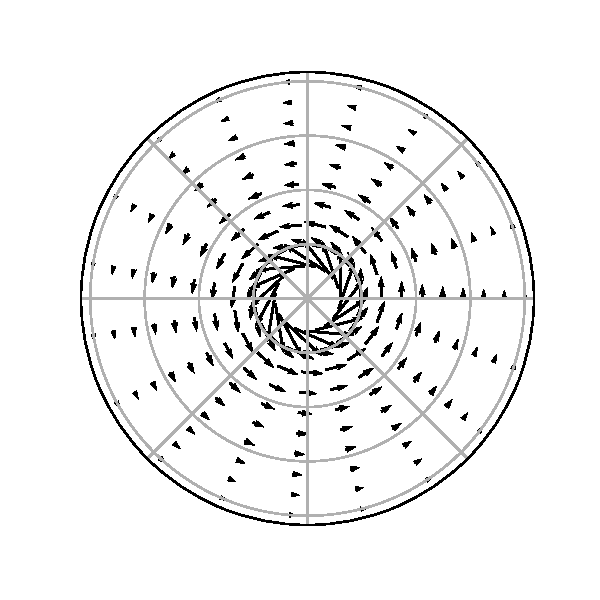
\includegraphics[width=0.5\linewidth]{Figures/Chapter1/fig_line_vortex_vector}
\caption{A line vortex flow, with $k = 1$.}
\label{fig_vortex}
\end{figure}

Despite these examples, vorticity really is related to the rotation of the flow -- but it's the \emph{local} rotation that it measures.  If we built a ``vorticity meter,'' using two pieces of plastic and marking one tip so we can see it, the difference between a globally rotating flow and the line vortex example is very noticeable; see Figure \ref{fig_vorticity_meter}.

\begin{figure}
\centering
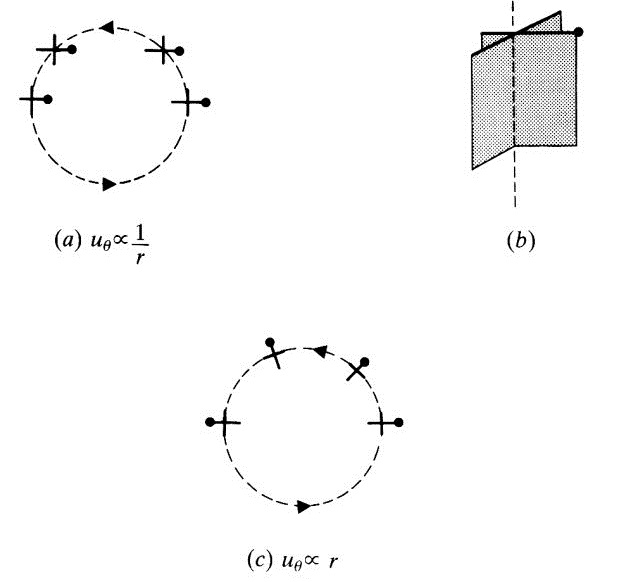
\includegraphics[width=0.7\linewidth]{Figures/Chapter1/fig_vorticity_meter.jpg}
\caption{A simple vorticity meter shows the difference between two rotating flows; it measures the \emph{local} rotation in a fluid. (Figure from \emph{Elementary Fluid Dynamics} by D. J. Acheson.) }
\label{fig_vorticity_meter}
\end{figure}

Finally, a bit of terminology: if the vorticity of a flow is zero, we say that it is \emph{irrotational}, so that
\begin{equation}
\boxed{
\boldsymbol{\nabla} \times \mathbf{u} = 0
}
\end{equation}
for an irrotational flow.





\section{Viscosity}
\label{sec_viscosity}

Experiment shows that a fluid doesn't ``slip'' along a boundary; instead, there is a thin boundary layer across which the flow speed drops smoothly and rapidly to zero (see Figure \ref{fig_boundary}).  The fluid elements in contact with the surface therefore move with the surface; this is called the \emph{no-slip condition}.

\begin{figure}
\centering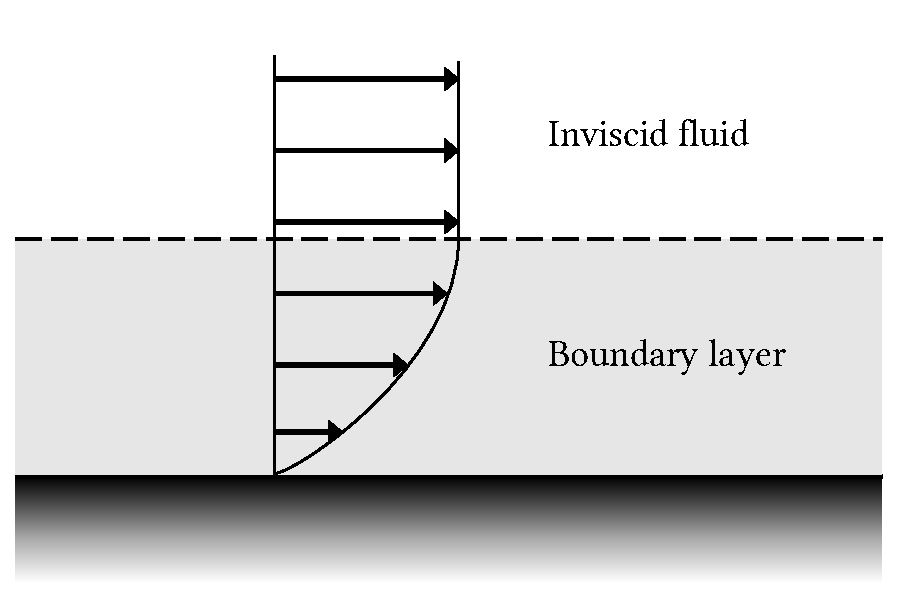
\includegraphics[width=0.7\linewidth]{Figures/Chapter1/fig_boundary_layer}
\caption{The boundary layer in a viscous fluid.  The arrow here represent the fluid velocity in the horizontal direction -- above the boundary layer, we can treat the fluid as inviscid, but within the velocity drops off to zero.}
\label{fig_boundary}
\end{figure}

The boundary layer comes from the viscosity of the fluid, which is defined (for so-called Newtonian fluids) via the tangential stress $\tau$,
\begin{equation}
\label{eq_visc_def}
\tau = \mu \frac{du}{dy}.
\end{equation}
We'll see where this comes from later on; for now, the quantity we want to focus on is the \emph{coefficient of viscosity} $\mu$.

Actually, we'll more frequently use the \emph{kinematic viscosity} $\nu$, defined by
$$
\nu \equiv \frac{\mu}{\rho},
$$
where $\rho$ is the density of the fluid. Some common viscosities (for a temperature of $15^\circ$C) are shown in Table \ref{tab_viscosity}.

\begin{table}[t]
\centering
  \begin{tabular}{l|l}
  & $\nu$ (cm$^2$/s) \\
  \hline \\
  Water & 0.01 \\
  Air & 0.15 \\
  Olive oil & 1.0 \\
  Glycerine & 18 \\
  Golden syrup & 1200
  \end{tabular}
  \caption{The viscosity of some fluids.}
  \label{tab_viscosity}
\end{table}

In some situations, the viscosity of a fluid can be neglected; we'll call the fluid \emph{inviscid} in that case:
\begin{equation}
\boxed{
\nu = 0
}
\end{equation}
for inviscid flow.  Even in situations where the viscosity is very small, though, the presence of the boundary layer can add significant complexity.  Because of the much larger velocity gradient within the boundary layer (where the fluid speed drops to zero  rapidly), the viscous stress becomes significant there, even when $\mu$ is normally small enough that we could neglect viscous effects elsewhere in the flow.

There's an additional feature of boundary layers that make them important dynamically -- in certain situations, they can actually separate from the boundary itself, causing the \emph{entire} flow to be quite different than that predicted by inviscid theory.  This is shown in Figure \ref{fig_boundary_sep} for low-viscosity flow past a cylinder.  Inviscid theory predicts the flow to the left, but boundary layer separation causes the flow on the right, where a large wake has developed past the cylinder.

\begin{figure}[t]
\centering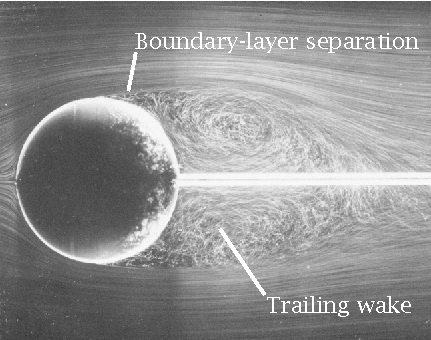
\includegraphics[width=0.5\linewidth]{Figures/Chapter1/fig_boundary_layer_sep.png}
\caption{Boundary layer separation occurring in flow past a smooth sphere.  (Photo adapted from \emph{An Album of Fluid Motion} by Milton Van Dyke.) }
\label{fig_boundary_sep}
\end{figure}

One way to characterize how important viscosity is to the flow dynamics is with the Reynolds number, defined by
\begin{equation}
R = \frac{UL}{\nu},
\end{equation}
where $U$ and $L$ are velocity and length scales characteristic to the flow (say, for example, the speed of an airplane and the width of its wing).  For large Reynolds number -- greater than a few thousand -- viscosity can be neglected, and the flow can become unstable and \emph{turbulent}.  Below this the flow is smooth, or \emph{laminar}, but viscosity effects can still usually be neglected.  For small Reynolds number, however -- less than one -- viscosity becomes important in how the fluid behaves.









\section*{Problems}
\addcontentsline{toc}{section}{Problems}

\begin{problem}[Streamlines]
Consider the flow given by 
\[
\uu = [x, x(x-1)(y+1), 0].
\]
Find an equation for the streamlines of the flow and plot them.
\end{problem}

\begin{problem}[ Unsteady flow]
\label{prob_unsteady}
Consider the \emph{unsteady} flow given by
\[
\mathbf{u} = [U, kt],
\]
where $U$ and $k$ are constants.  Show that the streamlines are straight lines at any particular point in time, and describe their behaviour as time goes on.  Then show that the path a fluid particle follows is parabolic rather than a straight line.  This is an example of how, for unsteady flow, fluid elements do not follow streamlines.

\end{problem}

\begin{problem}[Vector calculus practice]

Calculate the divergence and curl of the following vector fields.  State which flows are incompressible and which are irrotational (or both).

\begin{align*}
\text{(a) } & \mathbf{u} = [x^2, 3xz^2, -2xz] \\
\text{(b) } & \mathbf{u} = [xy, 2yz, 3zx] \\
\text{(c) } & \mathbf{u} = [y^2, 2xy+z^2, 2yz].
\end{align*}

\end{problem}

\begin{problem}[More vector calculus practice]
\label{prob_vc2}
Prove that the curl of a gradient  is always zero and that the divergence of a curl is always zero.

\end{problem}


\begin{problem}[Concentration of a pollutant]
Consider the flow about a stagnation point,
\[
\mathbf{u} = [\alpha x, -\alpha y],
\]
where $\alpha$ is a positive constant.  Suppose a pollutant is introduced into the fluid, and it's concentration is given by
\[
c(x, y, t) = \beta x^2 y e^{-\alpha t},
\]
for $y>0$, and where $\beta$ is a constant.  Does the pollutant concentration for any particular fluid element change with time?
\end{problem}

\begin{problem}[Acceleration of a rotating fluid]
A fluid in uniform rotation with angular velocity $\Omega$ is given by
\[
\uu = [-\Omega y, \Omega x, 0].
\]
Calculate the acceleration of the fluid and show that it can be written as
\[
-\Omega^2 \mathbf{r}.
\]
Is this acceleration what you expect?  Why or why not?
\end{problem}


\begin{problem}[Conservation of mass]
If the fluid is compressible, we can derive a condition to replace Equation \ref{eq_incompressibility} by assuming that mass must be conserved.  Use arguments similar to those in Section \ref{sec_incompressibility} to show that it implies
\begin{equation}
\frac{\partial \rho}{\partial t} + \div (\rho \uu ) = 0.
\end{equation}
Show also that, if the density is constant in space and time, this reduces to the usual incompressibility condition.
\end{problem}


\begin{problem}[Vorticity of a line vortex]
\label{prob_vortex_vorticity}
Show that the vorticity of a line vortex, 
\[
\uu = \frac{k}{r} \hat{\theta},
\]
is zero everywhere except at the origin, where it blows up.
\end{problem}



\begin{problem}[The Reynolds number]

Give an order of magnitude estimate of the Reynolds number for

(a) Flow past the wing of a Boeing 737 cruising at 150 m/s.

(b) A thick layer of golden syrup draining off a spoon.

(c) Air flowing through the trachea during normal breathing.

(d) Water flowing through a creek bed.

You'll have to estimate a speed and size for most of these.  Which could be turbulent?  Which would require viscous flow theory, and which inviscid theory?

\end{problem}


\chapter{Viscous Fluids}

%
% --- SECTION - THE NS EQ ---
% 

\section{The Navier-Stokes Equations}

We've discussed a lot of different flows -- about a stagnation point, a shear flow, a line vortex flow -- but we haven't yet talked about how we \emph{find} $\uu$.  That is, after all, the whole goal of fluid dynamics!

In short (and we'll come back to this in Section \ref{sec_ns_deriv} for a full derivation), fluid dynamics is governed by the Navier-Stokes equations,
\begin{equation}
\boxed{
\frac{D \uu}{Dt} = -\frac{1}{\rho} \grad p + \nu \nabla^2 \uu +  \mathbf{g}.
}
\end{equation}
We can recognize some of what's there -- the kinematic viscosity $\nu$ we've already talked about, and the acceleration is the left hand side.  In addition, there's also:
\begin{itemize}
\item The \emph{density} of the fluid, $\rho(\mathbf{x}, t)$.  If the fluid is incompressible, this is a constant in both space and time.
\item The \emph{pressure} of the fluid, $p(\mathbf{x}, t)$.  This is a scalar function and usually not uniform throughout the fluid.  Pressure is probably familiar to you, but we'll come back to it and properly define it when we derive the Navier-Stokes equations.
\item The gravitational field $\mathbf{g}$.  Usually -- but not always -- we'll be dealing with fluids at the surface of the Earth, and define our coordinate system so that $\mathbf{g} = [0,0,-g]$ where $g = 9.8$ m/s$^2$ as usual. 
\end{itemize}

The Navier-Stokes equations, named after Claude-Louis Navier and George Gabriel Stokes who (independently) derived them, are famously difficult to solve -- they're a set of coupled nonlinear second order partial differential equations.  In fact, showing that solutions to the Navier-Stokes equations always exist and are smooth is one of the seven ``Millennium Prize Problems'' from the Clay Mathematics Institute.  We won't be doing anything so difficult here; for some simple situations, the equations are readily solvable, even if they require some thought and a few tricks.


% SUBSECTION - CARTESIAN COORDS

\subsection{Cartesian Coordinates}

We'll begin with flows that are best described by the usual Cartesian coordinates $x$, $y$, and $z$.  In this coordinate system, the Navier-Stokes equations take on the form
\begin{align}
\label{eq_ns_cart1}
\dfdx{u}{t} + u\dfdx{u}{x} + v \dfdx{u}{y} + w \dfdx{u}{z} = -\frac{1}{\rho} \dfdx{p}{x} + \nu \left( \ddfdx{u}{x} + \ddfdx{u}{y} + \ddfdx{u}{z} \right) + g_x, \\
\dfdx{v}{t} + u\dfdx{v}{x} + v \dfdx{v}{y} + w \dfdx{v}{z} = -\frac{1}{\rho} \dfdx{p}{y} + \nu \left( \ddfdx{v}{x} + \ddfdx{v}{y} + \ddfdx{v}{z} \right) + g_y, \\
\dfdx{w}{t} + u\dfdx{w}{x} + v \dfdx{w}{y} + w \dfdx{w}{z} = -\frac{1}{\rho} \dfdx{p}{z} + \nu \left( \ddfdx{w}{x} + \ddfdx{w}{y} + \ddfdx{w}{z} \right) + g_z.
\end{align}

Furthermore, we'll assume our fluids are \emph{incompressible}, so that they must also satisfy the incompressibility condition, Equation \ref{eq_incompressibility}, which in Cartesian coordinates is
\begin{equation}
\label{eq_incomp_cart}
\dfdx{u}{x}  + \dfdx{v}{y} + \dfdx{w}{z} = 0.
\end{equation}

Those are an impressively complicated looking set of equations.  To solve them, however, we'll first make some assumptions based on the \emph{physical} nature of the problem we're examining; as we'll see in a moment, that will allow us to remove some terms and will simplify things considerably.

%
% --- SECTION - SIMPLE VISCOUS FLOWS ---
% 

\section{Simple Viscous Flows}


% SUBSECTION - STEADY POISEUILLE FLOW

\subsection{Poiseuille Flow in One Dimension}
\label{sec_poise_1d}

Consider fluid flowing steadily between two rigid boundaries, one at $y=0$ and one at $y = h$, under a constant pressure gradient 
\[
\frac{dp}{dx} = -P.
\]
Figure \ref{fig_poise_setup} shows the set-up and our coordinate system.

\begin{figure}
\centering
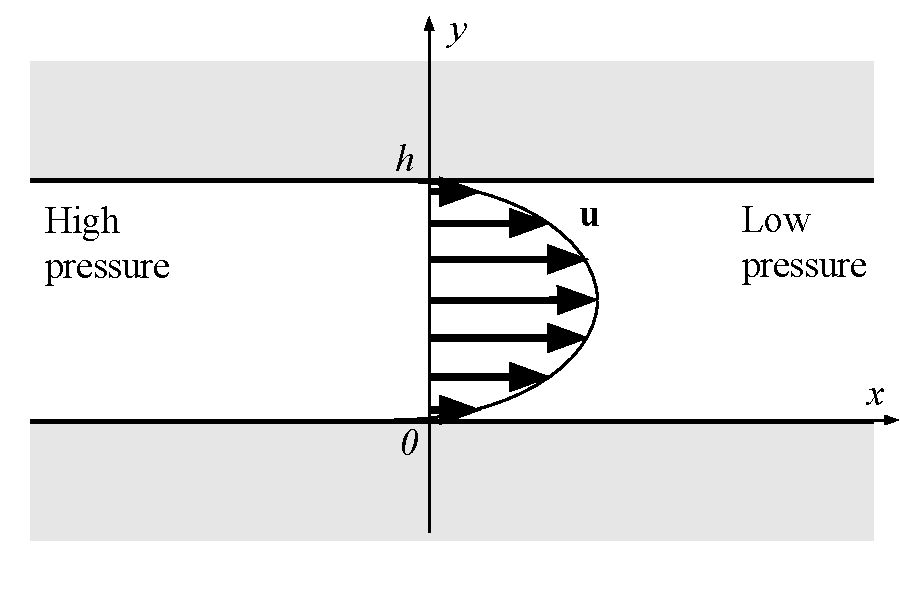
\includegraphics[width=0.7\linewidth]{Figures/Chapter2/fig_poise_setup}
\caption{The fluid will flow to the right due to the pressure gradient.}
\label{fig_poise_setup}
\end{figure}

This problem was first examined by Jean L\'eonard Marie Poiseuille, a physiologist interested in the flow of blood though capillaries and veins,\footnote{Actually, Poiseuille studied a slightly different problem -- see Problem \ref{prob_poise_cyl}.} although it also serves well as a model for air flowing through alveoli in lungs and fluid flowing through a straw.  It's also a great introduction to solving the Navier-Stokes equations, since it's essentially a one dimensional problem, as we'll see.  You can do the slightly more complicated two dimensional problem for homework (Problem \ref{prob_poise_2d}).

The first step to solving the Navier-Stokes equations is to examine symmetries and dependencies.  For example, this is clearly (at most) a two dimensional flow, with no dependence on $z$ or flow in the $w$ direction.  This assumes the ``walls'' at $y=0$ and $y=h$ are infinite in extent along the $z$-direction, but that's okay -- it still makes this problem a good approximation in more realistic (finite) situations.  This is also explicitly \emph{steady} flow, so there's no time dependence at all.  All this suggests we can write our the fluid velocity $\uu$ in terms of $x$ and $y$ only:
\[
\uu = [ u(x, y), v(x, y), 0].
\]

Furthermore, since the walls are also infinite in extent along the $x$-direction, we shouldn't expect any $x$-dependence in $\uu$.  If this seems surprising, consider moving our origin in Figure \ref{fig_poise_setup} left or right -- since the pressure gradient is \emph{constant}, exactly where we put the origin along the $x$-direction won't change the velocity at all.  So that means our flow dependence is now
\[
\uu = [u(y), v(y), 0].
\]
That's pretty simple, but we can do even better by looking at the incompressibility condition.  In our flow, $\partial u /\partial x = 0$ since the flow only depends on $y$, so Equation \ref{eq_incomp_cart} becomes
\[
\dfdx{v}{y} = 0.
\]
That means that $v$ is a constant.  But remember the no-slip condition from Section \ref{sec_viscosity} -- the walls are stationary, so the fluid in contact with them can't be moving either.  Since the velocity is zero at $y=0$, and $v$ is constant throughout the fluid, $v=0$ everywhere.

That last argument is a little tricky, but one we'll use quite a bit so go over again to make sure you get it.  The result, at the end of the day, is that for this situation, our flow takes on the form
\begin{equation}
\uu = [u(y), 0, 0].
\end{equation}
This is called steady \emph{plane-parallel shear flow}.  Although we derived this form specific to the situation shown in Figure \ref{fig_poise_setup}, it's applicable to others as well -- as long as the flow is two-dimensional, steady, and has that translational symmetry along the $x$-direction.

Now that we know exactly what variables the flow depends on, the Navier-Stokes equations get much simpler to write out (and solve!).  You should convince yourself that the $x$ component, Equation \ref{eq_ns_cart1}, becomes
\begin{equation}
\label{eq_poise_diffeq}
0 = -\frac{1}{\rho} \dfdx{p}{x} + \nu \ddfdx{u}{y}.
\end{equation}
Notice there's no gravity term here; I set $g_x = 0$. In fact, for simplicity I'll assume there is no gravity at all in this problem, so $g_y = g_z = 0$, too.  In Problem \ref{prob_poise_grav} you can see what effect gravity has on the situation, but it won't change the nature of it very much.  The other two Navier-Stokes equations just say that the pressure doesn't depend on $y$ or $z$, but we're already told that there is a constant pressure gradient in the $x$-direction, so that's nothing new.

Solving the differential equation in (\ref{eq_poise_diffeq}) is straightforward.  Let's write $dp/dx = -P$ and rearrange to get
\[
\frac{d^2u}{dy^2} = -\frac{P}{\nu \rho}.
\]
This is a second order ordinary differential equation which can be solved with two integrations to get
\[
u(y) = -\frac{P}{2\nu \rho} y^2 + c_1 y + c_2,
\]
where $c_1$ and $c_2$ are the two integration constants.

As usual, we can find the constants by applying our \emph{boundary conditions}.  In this case, we need the fluid at the boundary to have the same velocity as the boundary -- that's the no-slip condition again.  So, at the walls, we need
\[
u(0) = 0 \quad \text{and} \quad u(h) = 0.
\]
It follows from this that $c_2 = 0$ and
\[
c_1 = \frac{Ph}{2\nu \rho},
\]
and our final solution is
\begin{equation}
\label{eq_poise_steady}
u(y) = \frac{P}{2\nu \rho} (hy - y^2).
\end{equation}
The velocity profile is a parabola. 

How do we visualize this flow? Streamlines won't be any good here, since the flow is entirely in the $x$-direction -- the streamlines will just be horizontal.  Instead, we can plot the parabola directly on the system as shown in  Figure \ref{fig_poise_setup}, where I've also drawn in some representative vectors for the velocity $\uu$.  In this way we can see at a glance that the flow is strongest in the middle of the walls, and drops to zero at them according to the no-slip condition.



% SUBSECTION - Time Dependent Flow

\subsection{Time Dependent Flow}
\label{sec_poise_time}

The Poiseuille problem we just did is a great first example of solving the Navier-Stokes equations, but it's also an example of \emph{steady flow} -- nothing really changes in time. There are a few ways we can adapt this problem to introduce time dependence; we'll do two here, and you can do another one on your own if you like (Problem \ref{prob_poise_time}).

To add the time-dependence here we'll suppose that the steady flow we found in Section \ref{sec_poise_1d} has been going on for awhile, and at $t=0$ the pressure gradient stops suddenly:
\[
P = - \frac{dp}{dx} = 0 \quad \text{for} \quad t>0.
\]
What happens to the fluid for $t>0$?  Well, presumably it will slowly come to rest; how long does it take, and what does the flow look like until then?  To answer, we'll set up the problem the same way as above (Figure \ref{fig_poise_setup} again), with the boundaries at $y=0$ and $y=h$.  This is still a plane parallel shear problem, but now that we have time-dependence, the Navier-Stokes equation becomes a partial difference equation,
\begin{equation}
\label{eq_poise_pde}
\dfdx{u}{t} = \nu \ddfdx{u}{y}.
\end{equation}

Our boundary conditions are the same as before -- that $u = 0$ at the walls -- but the initial condition is our steady solution, Equation \ref{eq_poise_steady},
\begin{equation}
\label{eq_poise_ic}
u(y, t=0) = \frac{P}{2\nu \rho} (hy - y^2).
\end{equation}

To solve this partial differential equation, we'll use a tried and true method all physicists should know:  \emph{separation of variables}.  I'll assume here you're a little bit familiar with this technique,\footnote{If not, Griffiths' \emph{Introduction to Electrodynamics} is a great place to look; he has a whole section (3.3 in the third edition) devoted to it.} but I'll still go into enough detail to jog your memory.

To begin, we suppose that the solution, $u(y, t)$, can be written as the product of two single-variable functions:
\begin{equation}
u(y, t) = Y(y) T(t).
\end{equation}
If we plug this directly into Equation \ref{eq_poise_pde} -- noting that the partial derivatives treat one of the functions as a constant and act as an ordinary derivative on the other -- we get
\[
Y \frac{dT}{dt} = \nu T \frac{d^2Y}{dy^2}.
\]
We can rearrange this a bit to get this into a form where all the dependence on time is on the left hand side, and all the $y$-dependence is on the right,
\[
\frac{1}{\nu T} \frac{dT}{dt} = \frac{1}{Y} \frac{d^2Y}{dy^2}.
\]
The magic of separation of variables can now happen:  since $t$ and $y$ are independent variables -- you can change one without changing the other -- both sides of this equation must be constant!  If that weren't the case, we could change $t$ by a small amount, changing the left hand side, but leaving the right hand side the same -- and the two sides would no longer be equal.

Let's call the constant both sides are equal to $-k^2$; we'll see why it's negative in a moment, and why having it squared is a good idea.  In that case, separation of variables has turned our original partial differential equation into two ordinary differential equations:
\begin{align}
\frac{dT}{dt} & = -k^2 \nu T \\
\label{eq_poise_sho} 
\frac{d^2Y}{dy^2} & = -k^2 Y.
\end{align}

The first of these equations is easy to solve; rearrange to get
\[
\frac{dT}{T} = -k^2 \nu dt
\]
and integrate.  With a bit of work, we can write the solution as
\begin{equation}
T(t) = C e^{-k^2 \nu t},
\end{equation}
where $C$ is the integration constant.  We're not quite done with this yet, though -- we still don't know the value of $C$, or $k$ for that matter -- but let's move on to the second equation.  

Equation \ref{eq_poise_sho} one should look familiar,\footnote{If it doesn't, time to brush up on some of your mathematics -- having some familiarity with differential equations is necessary to be successful in learning fluid dynamics.} and it has the general solution
\[
Y(y) = A \sin (ky) + B \cos (ky).
\]
We can apply our boundary condition to this solution right away.  First, we need the fluid to be at rest along the bottom boundary at $y=0$; for that, we'll require $Y(0) = 0$.  If we evaluate the solution at $y=0$, we get $Y(0) = B$, meaning $B$ must be zero.  Our solution therefore becomes
\[
Y(y) = A \sin (ky).
\]
The second boundary condition is a little trickier.  Let's evaluate our solution at $y = h$:
\[
Y(h) = A \sin(kh).
\]
Somehow, this must equal zero as well.  One possibility is to make $A = 0$ -- but then $u = 0$, which doesn't make sense.  Same thing with setting $k = 0$.  But if we set 
\[
kh = n\pi, \quad n = 1, 2, 3, \dots,
\]
then that will work, since the zeros of the sine function are at every integer multiple of $\pi$.

This (almost) completes our full solution; combining $Y(y)$ with $T(t)$ to make the velocity, we get
\[
u(y, t) = Y(y)T(t) = A \sin (n\pi y / h) \, e^{-n^2 \pi^2 \nu t / h^2},
\]
where I've grouped both constants into $A$.  But wait!  This is actually an \emph{infinite} number of solutions, since $n$ is any integrer.  In fact, we can write down the \emph{general} solution to our original partial differential equation as a superposition of all of these individual solutions,
\begin{equation}
\label{eq_poise_sol}
u(y, t) = \sum_{n=1}^\infty A_n \sin(n \pi y / h) \, e^{-n^2 \pi^2 \nu t / h^2}.
\end{equation}
Note that the constant $A$ could be different in each term in the sum, so it has an index $n$ on it.

All we have left to do is find the values of the $A_n$s, which we do by using the initial conditions.  In fact, our solution can fit \emph{any} initial conditions we want; that's part of the magic of separation of variables.  If we evaluate Equation \ref{eq_poise_sol} at $t=0$ and equate it to our initial conditions, Equation \ref{eq_poise_ic}, we get
\[
\sum_{n=1}^\infty A_n \sin(n \pi y / h) =  \frac{P}{2\nu \rho} (hy - y^2).
\]
Somehow we have to solve this equation for $A_n$.  We can do that by application of what is sometimes called \emph{Fourier's trick}:\footnote{In fact, you might recognize these techniques as a part of the general theory of Fourier series.} we'll multiply both sides by $\sin(m \pi y/h)$ and integrate from $y=0$ to $y=h$, giving
\begin{equation}
\label{eq_poise_coeff}
\sum_{n=1}^\infty A_n \int_0^h \sin(m\pi y/h) \, \sin(n \pi y / h) \, dy =  \frac{P}{2\nu \rho} \int_0^h (hy - y^2)\sin(m\pi y/h) \, dy.
\end{equation}

Now, the left hand side turns out to be \emph{zero} if $n \neq m$; the two sine functions are called \emph{orthogonal} in that case.  In the case where $n=m$, the integral reduces to
\[
\int_0^h \sin^2(m \pi y / h) \, dy = \frac{h}{2}.
\]
We can combine these two results into one, using the Kronecker delta,
\begin{equation}
\delta_{mn} = \begin{cases} 0 \quad \text{if } m \neq n, \\ 1 \quad \text{if } m = n. \end{cases}
\end{equation}
Thus the left hand side of Equation \ref{eq_poise_coeff} becomes
\[
\sum_{n=1}^\infty A_n \int_0^h \sin(m\pi y/h) \, \sin(n \pi y / h) \, dy = \frac{h}{2} \sum_{n=1}^\infty A_n  \delta_{mn}.
\]
But the Kronecker delta will \emph{collapse} the sum -- every term in it will be zero except the $m$th one, so we get
\[
\frac{h}{2} \sum_{n=1}^\infty A_n  \delta_{mn} = \frac{h}{2} A_m.
\]

Phew!  That takes care of the left hand side, but we still have to do the right side.  That's a bit messy, since 
\[
\int_0^h (hy - y^2) \sin(m\pi y / h)\, dy = \frac{2h^3}{\pi^3 m^3} \left( 1 - \cos(m\pi) \right).
\]
Why messy?  Because the cosine evaluates to either $+1$ (if $m$ is even, and we get zero) or $-1$ (if $m$ is odd, and we get $2$).  That means we have to handle both of those cases separately.  Putting both sides of Equation \ref{eq_poise_coeff} together and solving for $A_m$ gives
\begin{equation}
A_m = \begin{cases}
       0, \quad & m \text{ even}, \\
       {4Ph^2}/{\pi^3 \nu \rho m^3}, \quad & m \text{ odd}.
\end{cases}
\end{equation}

Finally, we can write down our full solution to this problem.  Inserting this expression for $A_m$ into Equation \ref{eq_poise_sol} gives us
\begin{equation}
\label{eq_poise_time_sol}
u(y, t) = \frac{4Ph^2}{\pi^3 \nu \rho} \sum_{n=1, 3, 5 \dots}^\infty \frac{1}{n^3} \sin(n \pi y / h) \, e^{-n^2 \pi^2 \nu t / h^2}.
\end{equation}
That's not particularly nice looking answer, and it took us some work to get there, but we're done.  This gives us the fluid velocity at any time $t$ between the walls.

To take a look at the velocity, let's plot it up at a few times $t$, using the same convention we used in Figure \ref{fig_poise_setup}, where the distance along the $y$-direction is on the vertical axis, and the fluid velocity is along the horizontal.  Figure \ref{fig_poise_time} shows the flow at three times, one of which is $t=0$.  It's clear that, over time, the velocity does in fact go to zero.  If we want to estimate the length of time it takes to come to rest, we can look just at the $n=1$ term in the solution -- it's the dominant term, since each term after it gets smaller by a factor of $1/n^3$.  In that case, we can write the time factor as
\[
e^{-\pi^2 \nu t/h^2} = e^{-t/\tau},
\]
where $\tau = h^2/\pi^2 \nu$ is the characteristic time.  Thus the speed in the channel slows to about 37\% of its initial amount in a time $\tau$.  By a few characteristic times the fluid is practically at rest.

\begin{figure}
\centering
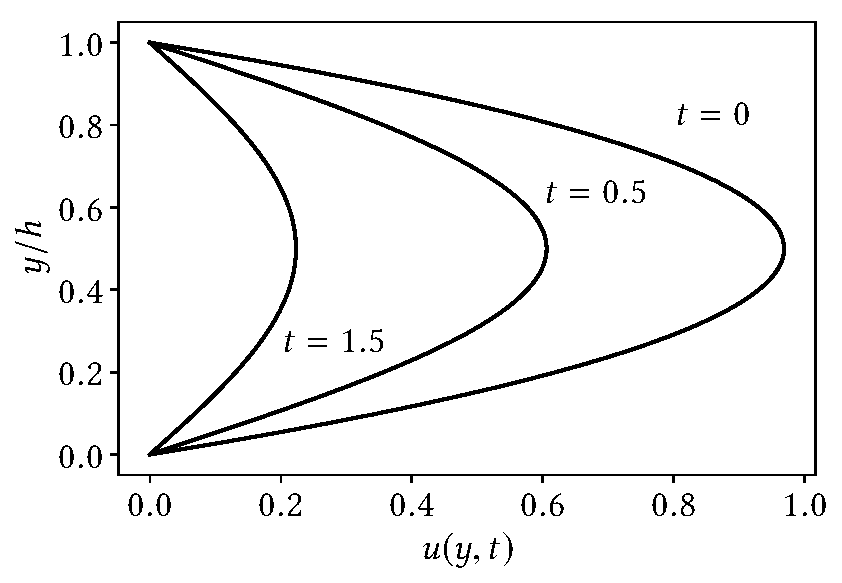
\includegraphics[width=0.7\linewidth]{Figures/Chapter2/fig_poise_time}
\caption{Poiseuille flow is slowing down over time once the pressure gradient shuts off. The velocity is in units of $4Ph^2 /\pi^3 \nu \rho$, and the time is in units of the characteristic time  $\tau = h^2 / \pi^2 \nu$. This plot used about 15 terms in the sum in Equation \ref{eq_poise_time_sol}.}
\label{fig_poise_time}
\end{figure}

% SUBSECTION - IMPULSIVE POISEUILLE FLOW

\subsection{An Impulsively Moved Boundary}
\label{sec_imp}

I'd like to do one more example with the two rigid boundaries before moving on -- mostly because in this example there's an interesting twist with how we'll have to solve the partial differential equation.


This time, we'll start with the fluid at rest in between the two boundaries; the set up is the same as in the above examples and  once again Figure \ref{fig_poise_setup} shows the coordinate system.  In this case, though, there won't be any pressure gradient -- we'll take $dp/dx = 0$ for the whole problem.  Once again, since nothing changes physically about the problem, we have a fluid dependent only on $y$ and flowing only in the $x$-direction, so this is still plane-parallel shear flow.  

We'll put the fluid in motion by, at $t = 0$,  suddenly \emph{jerking} the bottom boundary (the one at $y=0$)  -- we'll pull it to the right with constant speed $U$.  There won't be a period of acceleration here -- it's \emph{impulsively} moved and goes from at rest to moving instantaneously.  Thanks to the no-slip theorem, the bottom boundary will pull on the fluid elements in contact with it, which will in turn exert viscous forces on the fluid above, and so on.  To find out how the fluid responds to the impulsively moved boundary, we'll need to once again solve the Navier-Stokes equations.

They're identical, though, to the above time-dependent problem, Equation \ref{eq_poise_pde},
\begin{equation}
\label{eq_imp_diffeq}
\dfdx{u}{t} = \nu \ddfdx{u}{y}.
\end{equation}
The initial condition, however, is that the fluid starts at rest,
\begin{equation}
u(y, 0) = 0.
\end{equation}
The boundary conditions come from the no-slip condition, with the top boundary at rest but the bottom moving at constant velocity:
\begin{align}
u(0, t) & = U \quad \text{for } t>0, \\
u(h, t) & = 0.
\end{align}

To solve the differential equation (\ref{eq_imp_diffeq}), we'll once gain use technique of separation of variables.  However, there's a problem in this case -- the boundary condition is nonhomogeneous (since $u(0,t)$ is non-zero).  Unfortunately, separation of variables breaks down with nonhomogeneous boundary conditions (go ahead and try it on your own!).  

We can fix up the problem to deal with that, though, using a standard technique.  First, let's imagine that the flow is actually \emph{steady} -- there's no time dependence.  In that case, our equation simply becomes
\[
\frac{d^2 u_\text{steady}}{dy^2} = 0,
\]
which has the solution
\[
u_\text{steady}(y) = c_1 + c_2 y.
\]
To fit the boundary conditions, we need $c_1 = U$ and $c_2 = -U/h$, so we have
\[
u_\text{steady}(y) = U \left( 1 - \frac{y}{h} \right).
\]
This flow satisfies the differential equation and the boundary conditions, but not the initial conditions -- there's no time dependence at all.  However, it might be reasonable to think that, after a long time has passed, the flow will eventually reach a steady state like this.  In that case, it makes sense to write the \emph{full} solution as
\[
u(y, t) = u_\text{steady}(y) + u_1(y, t),
\]
where $u_1(y, t)$ is an unknown ``transient'' function; clearly, we want $u_1 \to 0$ as $t \to \infty$ so that we get our long-time steady state. 

If we plug this form of $u(y,t)$ into Equation \ref{eq_imp_diffeq}, our differential equation becomes
\begin{equation}
\dfdx{u_1}{t} = \nu \ddfdx{u_1}{y}.
\end{equation}
Notice that $u_\text{steady}$ has disappeared from the differential equation, and it looks like we've just swapped out $u$ for $u_1$.  What have gained?  Well, $u_1$ has different boundary conditions than $u$ -- notably, it now goes to zero at both $y=h$ \emph{and} $y=0$, where the steady state solution cancels the original condition -- and our boundary conditions are now homogeneous:
\begin{align}
u_1(0, t) & = 0 \quad \text{for } t>0, \\
u_1(h, t) & = 0.
\end{align}
The initial condition has also changed, since we need to cancel off the steady state term there, too:
\begin{equation}
\label{eq_poise_imp_ic}
u_1(y, 0) = -u_\text{steady} = -U \left( 1 - \frac{y}{h} \right).
\end{equation}

Now we're ready to solve by separation of variables.  The process and most of the steps are identical to what we just went over in Section \ref{sec_poise_time}, so I'll skip most of the details.  Thanks to the same differential equation and boundary conditions for $u_1$, the solution is once again
\[
u_1(y, t) = \sum_{n=1}^\infty A_n \sin(n \pi y / h) \, e^{-n^2 \pi^2 \nu t / h^2}.
\]
All that's left is to find the $A_n$s that fit the initial conditions, Equation \ref{eq_poise_imp_ic}.  Using Fourier's trick again (multiplying by $\sin(m \pi y / h)$ and integrating) leads to 
\[
A_n = -\frac{2U}{n\pi}.
\]
Finally, adding in the steady-state solution to get $u(y, t)$, we have
\[
u(y, t) = U \left[ 1 - \frac{y}{h} - \frac{2}{\pi} \sum_{n=1}^\infty \frac{1}{n} \sin(n \pi y / h) \, e^{-n^2 \pi^2 \nu t / h^2} \right].
\]

Figure \ref{fig_poise_imp} shows the fluid velocity $u(y,t)$ at a couple of different times.  The characteristic time is the same as in the previous problem; after a few $\tau = h^2/\pi^2 \nu$, the fluid reaches its steady state.


\begin{figure}
\centering
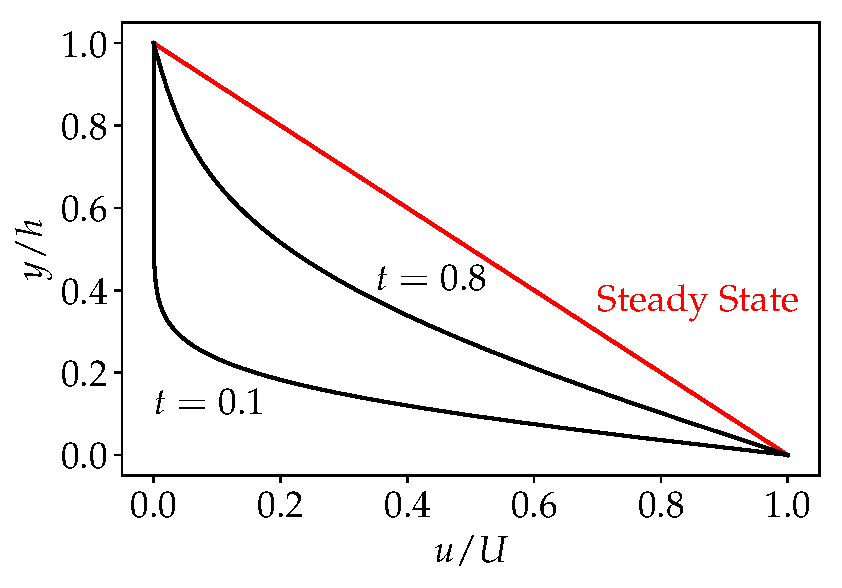
\includegraphics[width=0.7\linewidth]{Figures/Chapter2/fig_poise_imp}
\caption{A boundary suddenly jerked into motion will eventually move the fluid into a steady state.  The time is in units of the characteristic time $\tau$.}
\label{fig_poise_imp}
\end{figure}



% SUBSECTION - ONE BOUNDARY - SELF SIMILAR

\subsection{Self-Similar Flows}
\label{sec_self_similar}

The techniques we used to solve the three previous problems -- integrating an ordinary differential equation, using separation of variables to solve a partial differential equation, and then doing the same thing but with the added twist of using a steady state solution to handle nonhomogeneous boundary conditions -- are all standard techniques physicists use to solve differential equations.  All three problems also had very similar set-ups -- two boundaries and plane parallel shear flow.

I'd like to do one last example of time-dependent plane parallel shear flow before moving on to other kinds of situations, but this time I'll remove the boundary at $y=h$ -- we only have one boundary in this new problem, and it's along the $x$-axis.  Fluid exists only in the region $y>0$, but it can extend up to infinity -- see Figure \ref{fig_self_sim_setup}.

\begin{figure}
\centering
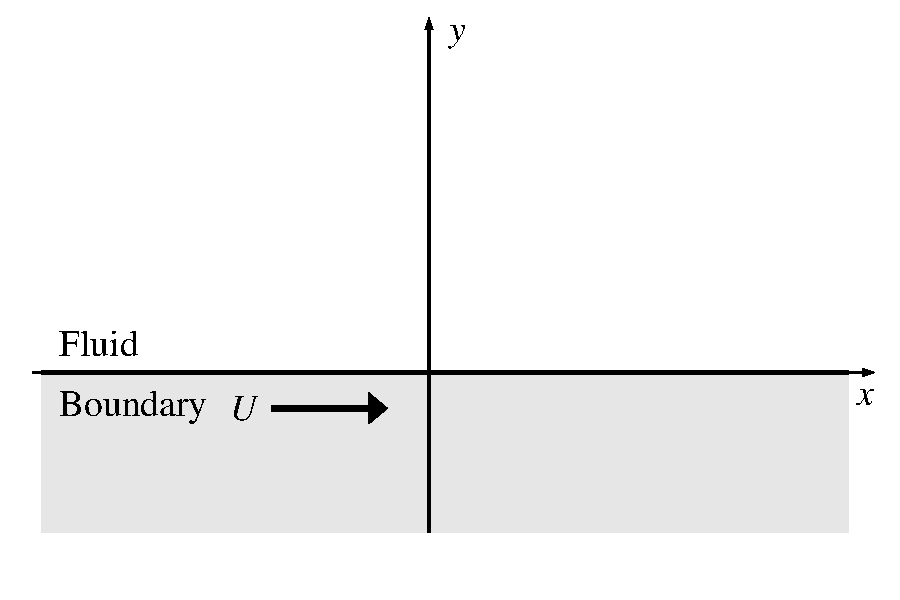
\includegraphics[width=0.7\linewidth]{Figures/Chapter2/fig_self_sim_setup}
\caption{A single boundary is suddenly jerked into motion.  This problem is \emph{self-similar} because it doesn't have a scale.}
\label{fig_self_sim_setup}
\end{figure}

As with the previous example, this boundary will be impulsively put into motion at $t=0$ with a velocity (to the right) of $U$.  We've already gone through the arguments in the last section about what kind of flow this is, and they all hold here, too -- the only difference is in the boundary conditions.  That means we once again have the partial differential equation
\begin{equation}
\label{eq_ss_diffeq}
\dfdx{u}{t} = \nu \ddfdx{u}{y}.
\end{equation}
to solve for our system.  The initial condition is just that the fluid is at rest, 
\begin{equation}
u(y, 0) = 0,
\end{equation}
and our usual no-slip condition at the boundary still applies,
\begin{equation}
u(0, t) = U.
\end{equation}
We have one other condition, as well, for the fluid far away from the boundary; this is where our problem will start to deviate from the others.  We'd expect that the motion of the boundary will affect the fluid above it, and this motion will propagate upward over time.  However, the fluid \emph{infinitely} far away will need an infinite amount of time to feel the motion of the boundary, which suggests that we require
\begin{equation}
\label{eq_ss_bc2}
u(\infty, t) = 0.
\end{equation}

Now, we could, if we wanted, go through the same procedure as before -- find a steady-state solution, apply separation of variables, and build our final answer as a superposition of solutions.  But that process is cumbersome (and we've already done it once!), and this problem can actually be solved in a completely different way, first done by Stokes.\footnote{This example is actually known as Stokes' first problem.}

Consider, first, some dimensional analysis.  Examining Equations \ref{eq_ss_diffeq}-\ref{eq_ss_bc2} we can see that our problem depends, at best, on four variables: $U$, $\nu$, $y$, and $t$.  But if we write the velocity as a non-dimensional variable,
\[
\tilde{u} = \frac{u}{U},
\]
then our differential equation becomes
\begin{equation}
\label{eq_ss_diffeq_tilde}
\dfdx{\tilde{u}}{t} = \nu \ddfdx{\tilde{u}}{y}.
\end{equation}
More importantly, our boundary condition at $y=0$ becomes
\[
\tilde{u}(0, t) = 1.
\]
This means that the solution for the non-dimensional $\tilde{u}$ can only depend on \emph{three} variables:  $\nu$, $y$, and $t$.  I'll write out the solution to the Navier-Stokes equation, then, as
\[
\tilde{u} = f(\nu, y, t),
\]
where $f$ is some unknown function.  We do know one thing about it, though:  since $\tilde{u}$ is dimensionless, so too must be $f$.

Okay, where are we going with this?  Well, since $f$ must be dimensionless, and since it can only depend on $\nu$, $y$, and $t$ and no other quantity, we need to rearrange those three variables into a combination that is dimensionless.  It turns out there is only \emph{one} way to do this, the combination
\[
\frac{y}{\sqrt{\nu t}}.
\]
All this is to suggest that, in our final solution to Equation \ref{eq_ss_diffeq_tilde}, $y$ and $t$ and $\nu$ can \emph{only} appear in the above combination.  This powerful idea will allow us to turn the partial differential equation into an ordinary one that we can integrate to solve -- much simpler than going through separation of variables.

This whole idea -- having the solution depend only on a dimensionless quantity -- is called \emph{self-similarity}, for reasons we'll see in a bit.  It's due to the fact that there is no \emph{physical scale} involved in the problem -- it doesn't involve a length scale at all, nor a time scale.  This is in contrast to the previous problem with a boundary at $y=h$ -- the value of $h$ sets the physical scale along the $y$-direction, and we wouldn't be able to write down a single combination of variables that was dimensionless in that case.  If you're finding it difficult to imagine the scale-free nature of the problem, imagine ``zooming'' in or out in Figure \ref{fig_self_sim_setup} -- because the fluid goes to infinity above the boundary, there's nothing to tell you that actually \emph{have} zoomed in or out, and the figure would look exactly the same.

Self-similarity is a powerful concept in fluid dynamics and many other fields, from mathematics to finance.  The most common example of it is probably the nature of some fractals, such as the Koch snowflake shown in Figure \ref{fig_koch}.  As you zoom in on the snowflake, the perimeter continues to look exactly the same.  A great example of a self-similar system in nature is the fronds on a fern, as shown in Figure \ref{fig_fern}.  Note that the overall structure of the fern is repeated on smaller scales, all the way down to the individual leaves.  As we'll see, along with the scale-free situation, our solution to this problem will also be self-similar in the same way.

\begin{figure}
\centering
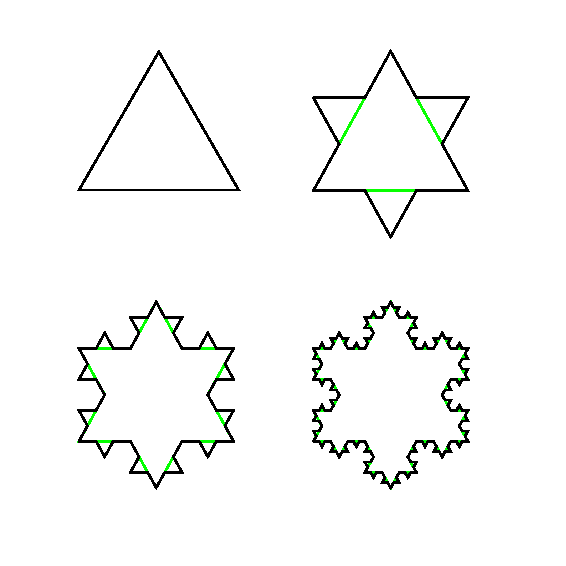
\includegraphics[width=0.5\linewidth]{Figures/Chapter2/fig_koch}
\caption{The procedure for constructing a Koch snowflake, a good example of exact self-similarity.  \href{https://commons.wikimedia.org/wiki/File:KochFlake.svg}{Image by Wxs / CC BY-SA 3.0.} }
\label{fig_koch}
\end{figure}

\begin{figure}
\centering
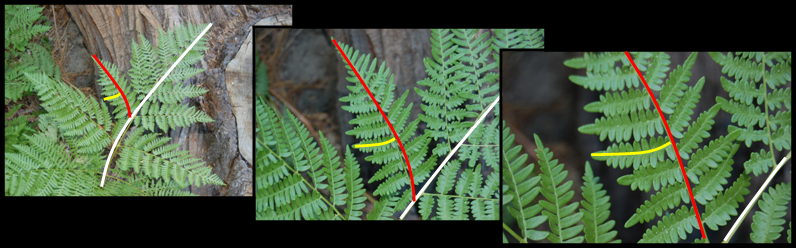
\includegraphics[width=1\linewidth]{Figures/Chapter2/fig_fern.png}
\caption{A fern is an example of self-similarity found in nature.  \href{https://www.flickr.com/photos/78523101@N04/7572281628}{Photo by Jason Hine / CC BY-NC 2.0.} }
\label{fig_fern}
\end{figure}

It's time to exploit this idea mathematically.  Let's define a new variable,
\begin{equation}
\eta = \frac{y}{\sqrt{\nu t}}.
\end{equation}
Our goal will be to rewrite the partial differential equation (\ref{eq_ss_diffeq_tilde}) in terms of $\eta$ rather than $y$ and $t$.  We can do this with the chain rule, so that
\[
\dfdx{\tilde{u}}{t} = \frac{df}{d\eta} \dfdx{\eta}{t} = -\frac{y}{2 \nu^{1/2} t^{3/2}} f',
\]
where the prime indicates a derivative with respect to $\eta$, and
\[
\ddfdx{\tilde{u}}{y} = \frac{d^2 f}{d\eta^2} \left( \dfdx{\eta}{y} \right)^2 + \dfdx{f}{\eta} \ddfdx{\eta}{y} = \left( \frac{1}{\nu t} \right) f''.
\]
Careful with the second derivative calculation -- it uses a product rule as well as the chain rule, so go over it yourself to make sure you known where the terms come from.  Plugging these two derivatives back into Equation \ref{eq_ss_diffeq_tilde} gives, after a bit of rearranging,
\begin{equation}
f'' + \frac{1}{2} \eta f' = 0.
\end{equation}
As promised, we now have only one ordinary differential equation to worry about -- and note that this equation contains only dimensionless quantities.

It's straightforward to solve this differential equation as well.  First, let
\[
g = f',
\]
so that $g' = f''$, and the equation becomes the first order
\[
g' + \frac{1}{2} \eta g = 0.
\]
Writing all the $g$s on one side and the $\eta$s on the other allows us to integrate it, to get
\[
g(\eta) = f' = B e^{-\tfrac{1}{4} \eta^2},
\]
where $B$ is the integration constant.  Integrating one more time will get us $f(\eta$),
\[
f(\eta) = A + B \int_0^\eta e^{-\tfrac{1}{4} \eta'^2} \, d\eta'.
\]
Here, $A$ is another integration constant (to account for the definite integral), and I've written $\eta'$ as the integration variable to avoid confusion.  Unfortunately, actually solving the integral in this equation is not possible in closed form -- in fact, the integral
\[
\frac{1}{\sqrt{\pi}} \int_0^x e^{-\tfrac{1}{4} u^2} du \equiv \text{erf}(x),
\]
is called the \emph{error function}, and is used extensively in probability and statistics.  Since we can only evaluate the error function numerically, I'll continue to just write out the integral.

We can find the constants $A$ and $B$ with our boundary conditions and the initial condition.  Before we do that, though, we need to express them in terms of $\eta$ rather than $y$ and $t$.  The first boundary condition is
\[
\tilde{u}(0, t) = 1.
\]
But at this place ($y=0$) and time ($t$), we have $\eta = 0$,  so the boundary condition for $\eta=0$ becomes
\[
f(0) = 1.
\]
The second boundary condition likewise becomes
\[
f(\infty) = 0.
\]
Also, recall that the initial condition was $\tilde{u}(y, 0) = 0$.  In this case, $\eta \to \infty$, since $t$ is in the denominator, and we get again the same expression as the second boundary condition -- as expected, we have only two boundary conditions for our second order differential equation.

Using these two boundary conditions leads to $A=1$ and $B = -1/\sqrt{\pi}$.  We can write our final solution, then (using $u = U\tilde{u}$), as
\begin{equation}
u(y, t) = f(\eta) = U\left[ 1 - \frac{1}{\sqrt{\pi}} \int_0^\eta e^{-\tfrac{1}{4} \eta'^2} d\eta' \right],
\end{equation}
where, of course, $\eta = y / \sqrt{\nu t}$.

We can take a look at the velocity for a couple of different times to see how the fluid responds to the impulsively moved boundary -- see Figure \ref{fig_ss_vel1}.  As expected, at later time the fluid is moving faster, and \emph{more} of the fluid is moving.  This is evident in Figure \ref{fig_ss_vel1}; at $t=1$, the fluid above $y \sim 3$ practically isn't moving, while for $t=10$, the motion of the fluid extends up to $y \sim 10$.

\begin{figure}
\centering
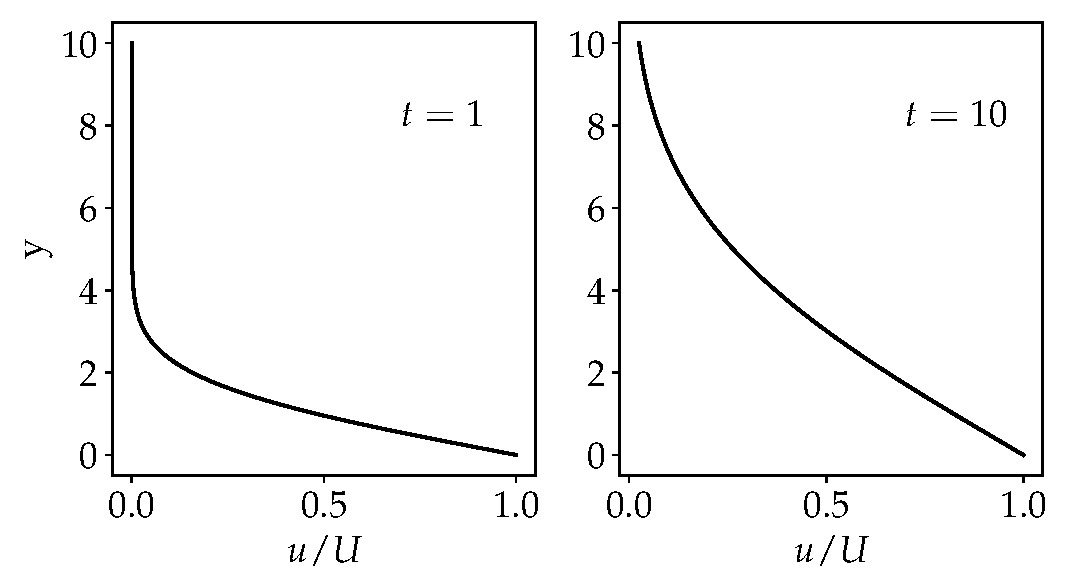
\includegraphics[width=0.8\linewidth]{Figures/Chapter2/fig_ss_vel1}
\caption{The fluid velocity for an impulsively moved boundary at $y=0$.  Note how long it takes for the fluid to respond -- at the later time on the right (ten times longer than the left), the velocity has increased at all points but still drops to zero around $y=10$.  I set $\nu = 1$ for convenience. }
\label{fig_ss_vel1}
\end{figure}

I mentioned earlier that this solution would be self-similar, but that's not very noticeable in Figure \ref{fig_ss_vel1}.  That's because both time \emph{and} space must be scaled together to get the same velocity curve.  In fact, if we zoom out on the $y$-axis as we move forward in time, the motion of the fluid should always be the same.  We can see that in Figure \ref{fig_ss_vel2}, which changes the scale of the $y$-axis for the right-hand plot at $t=10$.  Rather than going from $y=0$ to $y=10$, as in Figure \ref{fig_ss_vel1}, we go from $y=0$ to
\[
y = {10}{\sqrt{\nu t}}
\]
(remember, $\eta = y / \sqrt{\nu t}$).  Thus, as $t$ changes, so too does the scale of $y$.  In this case, both velocity curves look identical, and the solution is self-similar.

\begin{figure}
\centering
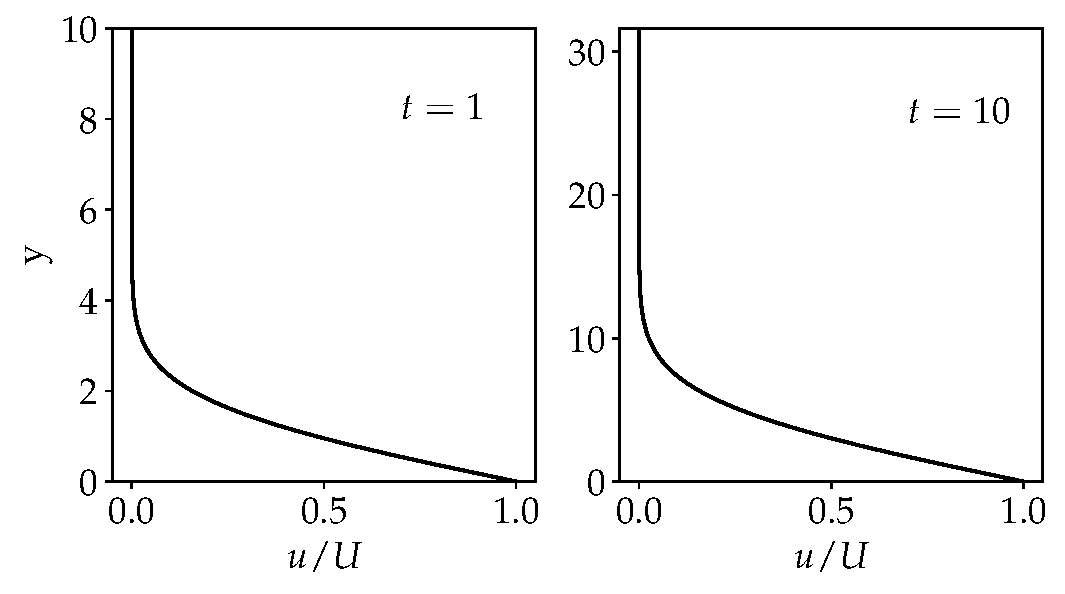
\includegraphics[width=0.8\linewidth]{Figures/Chapter2/fig_ss_vel2}
\caption{The fluid velocity for an impulsively moved boundary at $y=0$.  This time, I've changed the $y$-axis scale so that the two curves are self-similar.}
\label{fig_ss_vel2}
\end{figure}


%
% --- SECTION - CIRCULAR FLOW ---
% 

\section{Circular Flow}


% SUBSECTION - THE NS EQs IN CYLINDRICAL

\subsection{The Navier-Stokes Equations in Cylindrical Coordinates}
\label{sec_ns_cyl}

The Navier-Stokes equations are trickier to write down in cylindrical coordinates, mainly due to the fact that the cylindrical unit vectors $\hat{r}$ and $\hat{\theta}$ in Equation \ref{eq_u_cyl} are not \emph{constant} -- they depend on $\theta$:
\begin{align*}
\hat{r} & = \cos \theta \hat{i} + \sin \theta \hat{j} \\
\hat{\theta} & = - \sin \theta \hat{i} + \cos \theta \hat{j}.
\end{align*}
When evaluating the derivatives in the Navier-Stokes equation, then, you have to be very careful to take this dependence into account.  For example, note that
\[
\frac{d\hat{r}}{d\theta} = \hat{\theta}
\]
and
\[
\frac{d\hat{\theta}}{d\theta} = - \hat{r}.
\]

Furthermore, the gradient and Laplacian operators in cylindrical coordinates are a little more cumbersome than in Cartesian; I won't bother writing them out here, but you should look them up on your own.\footnote{I really like the front and back covers in Griffiths' \emph{Introduction to Electrodynamics} for this.}  Altogether, here's the Navier-Stokes equations in cylindrical coordinates for you:
\begin{align}
\label{eq_ns_r}
\frac {\partial u_{r}}{\partial t} + (\mathbf{u} \cdot \grad) u_{r} - \frac {u_{\theta}^{2}}{r} & = - \frac {1}{\rho} \frac {\partial p}{\partial r} + \nu \left (\nabla^{2} u_{r} - \frac {u_{r}}{r^{2}} - \frac {2}{r^{2}} \frac {\partial u_{\theta}}{\partial \theta} \right) +  g_r\\
\label{eq_ns_theta}
\frac {\partial u_{\theta}}{\partial t} + (\mathbf{u} \cdot \grad) u_{\theta} + \frac {u_{r} u_{\theta}}{r} & = - \frac {1}{\rho r} \frac {\partial p}{\partial \theta} + \nu \left (\nabla^{2} u_{\theta} - \frac {u_{\theta}}{r^{2}} + \frac {2}{r^{2}} \frac {\partial u_{r}}{\partial \theta} \right) + g_\theta\\
\label{eq_ns_z}
\frac {\partial u_{z}}{\partial t} + (\mathbf{u} \cdot \grad) u_{z} & = -\frac {1}{\rho} \frac {\partial p}{\partial z} + \nu \nabla^{2} u_{z} + g_z \\
\end{align}
where
\begin{align}
(\mathbf{u} \cdot \grad) & = u_{r} \frac {\partial}{\partial r} + \frac {u_{\theta}}{r} \frac {\partial}{\partial \theta} + u_{z} \frac {\partial}{\partial z}, \\
\nabla^{2} & = \frac {1}{r} \frac {\partial}{\partial r} \left (r \frac {\partial}{\partial r} \right) + \frac {1}{r^{2}} \frac {\partial^{2}}{\partial \theta^{2}} + \frac {\partial^{2}}{\partial z^{2}}.
\end{align}
In addition, the incompressibility condition $\div \uu = 0$ becomes 
\begin{equation}
\frac {1}{r} \frac {\partial}{\partial r} (r u_{r}) + \frac {1}{r} \frac {\partial u_{\theta}}{\partial \theta} + \frac {\partial u_{z}}{\partial z} = 0.
\end{equation}


% SUBSECTION - UNIFORMLY ROTATING FLUID

\subsection{Uniformly Rotating Fluid}

For our first problem, we'll consider fluid within a cylinder of radius $a$, as shown in Figure \ref{fig_cyl_setup}, with the cylinder rotating with an angular speed of $\Omega$. 

Already this is two dimensional flow -- we'll assume the cylinder is infinitely long, so there won't be any $z$ dependence of flow in that direction.  But, to make things simpler, we also impose full cylindrical symmetry on our flow:  the velocity will always take the form
\begin{equation}
\uu = u_\theta (r, t) \, \hat{\theta}.
\end{equation}
This means that the flow is always \emph{circular}, with streamlines that are circles.  Furthermore, the speed of the fluid only depends on the distance $r$ from the origin, giving us the cylindrical symmetry.  One nice benefit to a flow of this form is that the incompressibility condition is automatically satisfied, which you can check yourself with Problem \ref{prob_cyl_incomp}.

\begin{figure}
\centering
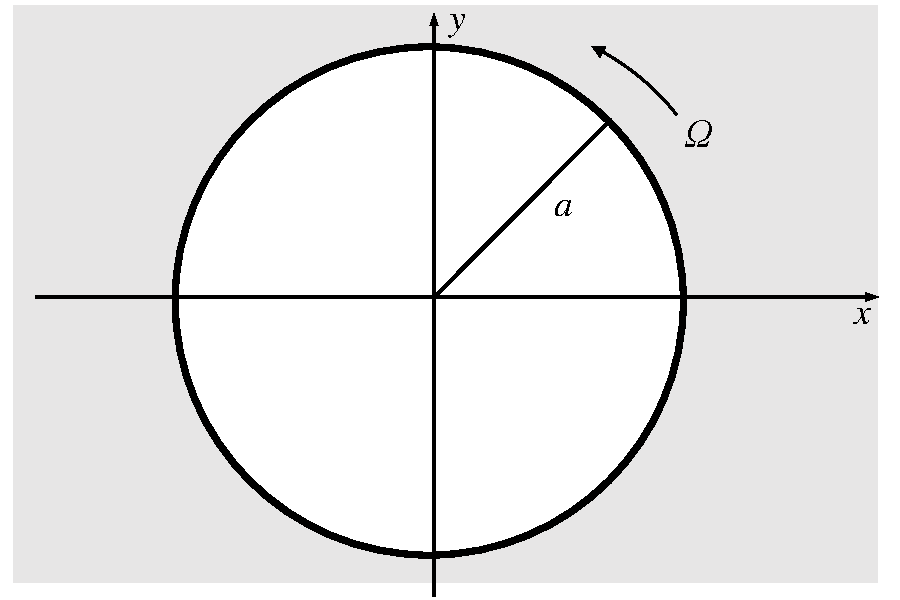
\includegraphics[width=0.7\linewidth]{Figures/Chapter2/fig_cyl_setup}
\caption{The fluid is constrained to be within a cylinder of radius $a$.  We'll put the origin at the centre of the cylinder.}
\label{fig_cyl_setup}
\end{figure}

As you might expect, taking this form of the velocity drastically reduces the Navier-Stokes equations.  Equations \ref{eq_ns_r} - \ref{eq_ns_z} become
\begin{align}
\frac{u_\theta^2}{r} & = \frac{1}{\rho} \dfdx{p}{r} \\
\label{eq_ns_theta2}
\dfdx{u_\theta}{t} & = -\frac{1}{\rho r} \dfdx{p}{\theta} + \nu \left( \ddfdx{u_\theta}{r} + \frac{1}{r} \dfdx{u_\theta}{r} - \frac{u_\theta}{r^2} \right) \\
\label{eq_ns_z2}
0 & = -\frac{1}{\rho} \dfdx{p}{z}.
\end{align}
Note that I've completely dropped the gravity terms here -- but see Problem \ref{prob_poise_grav} for the minimal effect that gravity has on our problems.

Now, the third equation above -- the one for $z$ -- just says that the pressure $p$ doesn't depend on $z$ at all, not surprising given the symmetry of the problem.  The first equation gives us a relationship between the fluid velocity $u_\theta$ and the radial pressure gradient, so if we know one we can get the other.  The second equation is the important one, but we can clean it up a bit more.  

Since $u_\theta = u_\theta(r, t)$ only, Equation \ref{eq_ns_theta2} says that $\partial p / \partial \theta$ must also be a function of only $r$ and $t$.  So we can write
\[
\dfdx{p}{\theta} = P(r, t),
\]
where $P(r, t)$ is some unknown function.  If we integrate this to find $p$, we get
\[
p = P(r, t) \theta + f(r, t),
\]
where $f(r, t)$ is the integration ``constant'' -- remember, we have a partial derivative here (and note that there's no $z$ dependence thanks to Equation \ref{eq_ns_z2}).  But this shows us that the function $P(r, t)$ \emph{must} be zero, since otherwise the pressure would be a multivalued function of position; it would take on different values for $\theta = 0$ and $\theta = 2 \pi$, for example, even though those two angles represent the same point in space.

Equation \ref{eq_ns_theta2} then becomes, with $P(r, t) = \partial p / \partial \theta = 0$, 
\begin{equation}
\label{eq_ns_evol}
\boxed{
\dfdx{u_\theta}{t} =  \nu \left( \ddfdx{u_\theta}{r} + \frac{1}{r} \dfdx{u_\theta}{r} - \frac{u_\theta}{r^2} \right).
}
\end{equation}
This equation determines the evolution of the fluid velocity.

Now we can go back to our original problem -- fluid inside a rotating cylinder.  We'll first assume the fluid is \emph{steady}, so that $\partial u_\theta / \partial t = 0$.  Multiplying Equation \ref{eq_ns_evol} by $r^2$ gives us
\begin{equation}
\label{eq_spin_diffeq}
r^2 \frac{d^2 u_\theta}{dr^2} + r \frac{d u_\theta}{dr} - u_\theta = 0.
\end{equation}
Notice that the viscosity has dropped out of the problem.  To solve this ordinary differential equation, let's ``guess'' at a power-law solution of the form
\[
u_\theta(r) = r^m.
\]
Plugging this form into our equation leads to the quadratic 
\[
m^2 -1 = 0,
\]
which has roots $m = +1$ and $m = -1$.  Our general solution is then
\begin{equation}
\label{eq_cyl_steady_gen_sol}
u_\theta (r) = Ar + \frac{B}{r}.
\end{equation}

Since we have viscous fluid, one of our boundary conditions must be that the fluid moves with the same velocity as the cylinder wall, so that
\[
u_\theta(a) = \Omega a.
\]
We don't really have another boundary condition, since there isn't another boundary; however, note that the second term in Equation \ref{eq_cyl_steady_gen_sol} blows up at $r=0$, the centre of the cylinder.  So, to keep the fluid velocity everywhere finite, we need to set $B = 0$.  The boundary condition then leads to $A = \Omega$, so our solution is 
\begin{equation}
\label{eq_cyl_steady_sol}
u_\theta (r) = \Omega r.
\end{equation}
This flow is in \emph{solid body rotation} -- in other words, the fluid rotates in exactly the same way as a solid body would, at constant angular speed $\Omega$.


% SUBSECTION - SPIN DOWN

\subsection{Spin Down of Rotating Fluid}

What happens to the fluid if the rotating cylinder is suddenly brought to rest?  Now we have time-dependent flow, and we'll have to use the full Equation \ref{eq_ns_evol} to model what happens.  Just a warning before we proceed:  this is a pretty complicated problem to solve, and will require some knowledge about Bessel functions.  We'll take it slow, but it might help to ready up on them first.

We'll use separation of variables to solve the partial differential equation, but first we should write out the initial and boundary conditions.  The initial condition is of course our steady state solution we just found, Equation \ref{eq_cyl_steady_sol},
\begin{equation}
\label{eq_spin_ic}
u_\theta (r, t=0) = \Omega r.
\end{equation}
We'll suppose the cylinder is brought to rest at $t=0$, so after that the no-slip condition says that
\begin{equation}
u_\theta(a, t) = 0 \quad \text{for } t > 0.
\end{equation}
As with our last problem, we'll also have to make sure that the velocity is finite everywhere in the fluid.

Let
\[
u_\theta(r, t) = R(r) T(t)
\]
and plug that into Equation \ref{eq_ns_evol}.  Dividing both sides by $RT$ gives
\[
\frac{1}{\nu T} \frac{dT}{dt} = \frac{1}{R} \frac{d^2R}{dr^2} + \frac{1}{rR} \frac{dR}{dr} - \frac{1}{r^2}.
\]
The left hand side is a function of time $t$ only, while the right hand side depends only on $r$.  Since they're independent variables, both sides must be equal to a constant, which, with the benefit of hindsight, we'll call $-k^2$.

The left hand side becomes
\[
 \frac{dT}{dt} = -\nu k^2 T,
\]
which has the solution
\begin{equation}
T(t) = C e^{-\nu k^2 t},
\end{equation}
where $C$ is a constant.  The right hand side is a little more difficult.  With a little manipulation (multiplying both sides by $r^2 R$) we can write it as
\[
r^2 \frac{d^2R}{dr^2} + r\frac{dR}{dr} + \left( k^2 r^2 - 1 \right) R = 0.
\]
One more small change:  let 
\[
x = k r.
\]
Then the equation becomes
\begin{equation}
\label{eq_bessel}
x^2 \frac{d^2R}{dx^2} + x\frac{dR}{dx} + \left(  x^2 - 1 \right) R = 0.
\end{equation}
This equation isn't easy to solve by hand, but it turns out to be a fairly famous differential equation that pops up in various places in physics (like electromagnetism and acoustics) -- it's called Bessel's equation, and the solutions are called \emph{Bessel functions}.

The Bessel function of the first kind is usually written $J_\alpha(x)$, where $\alpha$ is called the \emph{order} of the Bessel function.  In our case, with the $(x^2 - 1)$ term in the equation, we're dealing only with the first order, so $\alpha = 1$.  The second solution is the Bessel function of the second kind, sometimes called the Neumann function, $Y_\alpha(x)$.  We can't write either function in closed form -- the best we can do is a series solution -- but I've plotted both $J_1(x)$ and $Y_1(x)$  in Figure \ref{fig_bessel}.  Note that both functions are oscillatory, but not with a nice regular period like sine and cosine; Table \ref{tab_bessel} lists a few of the zeros of each, and we'll need those in a moment.

\begin{figure}
\centering
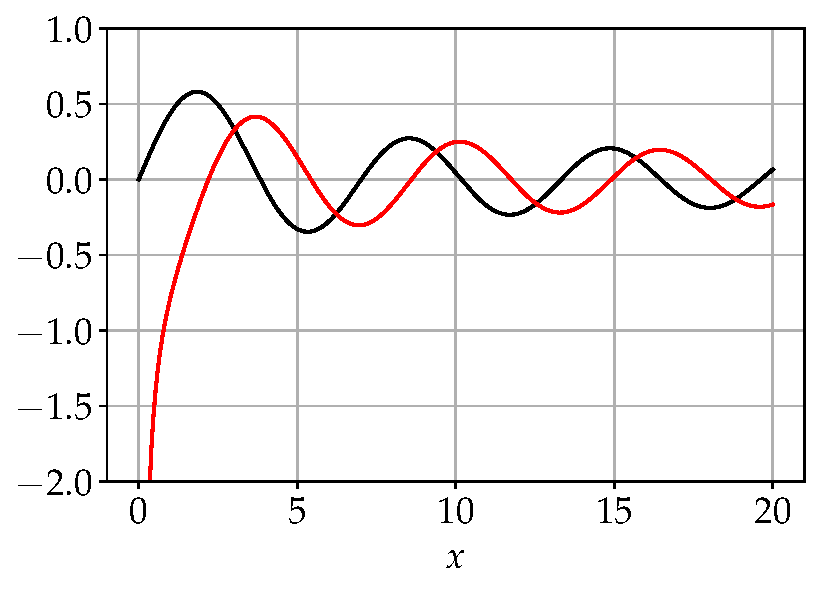
\includegraphics[width=0.7\linewidth]{Figures/Chapter2/fig_bessel}
\caption{The Bessel functions of the first (black) and and second (red) kind, of order $\alpha = 1$.}
\label{fig_bessel}
\end{figure}

\begin{table}[t]
\centering
  \begin{tabular}{l|l|l}
  & $J_1(x)$ & $Y_1(x)$ \\
  \hline \\
   $\lambda_1$ & 3.83170597   & 2.19714133    \\
   $\lambda_2$ & 7.01558667 & 5.42968104   \\
   $\lambda_3$ & 10.17346814 & 8.59600587  \\
   $\lambda_4$ & 13.32369194 & 11.74915483 \\
   $\lambda_5$ & 16.47063005 & 14.89744213
  \end{tabular}
  \caption{The first five zeros for the Bessel functions.}
  \label{tab_bessel}
\end{table}

The general solution to Equation \ref{eq_bessel} is the superposition of both Bessel functions, 
\[
R(x) = A J_1(x) + B Y_1(x).
\]
However, we can see from Figure \ref{fig_bessel} that the second function goes to negative infinity at the origin.  This is no good -- we want the velocity of the fluid to always be finite -- so we can drop the this function and set $B=0$.  Going back to using $r$ instead of $x$, we have
\[
R(r) = A J_1(kr).
\]

Now we can apply our boundary condition at $r=a$.  I'll write it out for you:
\[
R(a) = A J_1 (ka) = 0.
\]
Clearly, we can't set $A=0$, since that will give us a static fluid; instead, we'll have to use the fact that the Bessel function has an infinite number of zeros, just like we did with the sine function back in Section \ref{sec_imp}.  Unfortunately, the Bessel zeros aren't at nicely periodic locations like $n\pi$; as you can see in Table \ref{tab_bessel}, they're neither periodic nor at nice locations.  Instead, we'll have to be more general, so I'll call the $n$th zero of the Bessel function $\lambda_n$.  That is, 
\[
J_1(\lambda_n) = 0
\]
for every value of $\lambda_n$.  The boundary condition thus implies that $ka = \lambda_n$, or
\[
k = \frac{\lambda_n }{a}.
\]

Let's put our solution so far together.  We'll combine the results for $T(t)$ and $R(r)$ to get the fluid velocity
\[
u_\theta(r, t) = R(r) T(t) = A \, J_1(\lambda_n r / a) \, e^{-\lambda_n^2 \nu t /a^2},
\]
where I've combined the two constants into $A$.  As is usual with separation of variables, we end up with not just \emph{one} solution, but an \emph{infinite} number of them.  That means the most general solution is a linear combination of all of them,
\begin{equation}
u_\theta(r, t) = \sum_{n=1}^\infty A_n \, J_1(\lambda_n r / a) \, e^{-\lambda_n^2 \nu t /a^2}.
\end{equation}

Even though we've been dealing with Bessel function, the process of separation of variables is the same as we went through in Section \ref{sec_poise_time} -- if you can follow that discussion, you should be okay here, too.  We just have one more step:  finding the values of the constants $A_n$ that will match our initial conditions.  This part is similar to before, too, but does require a bit of advanced knowledge of Bessel functions, so watch carefully.

Our initial conditions, from Equation \ref{eq_spin_ic} say
\begin{equation}
\label{eq_spin_ic2}
u_\theta(r,0) =  \sum_{n=1}^\infty A_n \, J_1(\lambda_n r / a) = \Omega r.
\end{equation}
Just like sinusoidal functions, Bessel functions are orthogonal, although it looks a little different; it turns out that\footnote{See, for example, Arfken and Weber's \emph{Mathematical Methods for Physicists}, Fourth Edition, p. 646.}
\[
\int_0^a J_1(\lambda_n r / a) J_1(\lambda_m r /a) \, r\, dr = 0
\]
if $m \neq n$.  If $m = n$, then the result is
\[
\int_0^a J_1^2(\lambda_n r / a) \, r \, dr = \frac{a^2}{2} J_2^2(\lambda_n)
\]
(notice that's the second order Bessel function showing up on the right hand side).

We can use these results to solve for the $A_n$s.  Multiply both sides of Equation \ref{eq_spin_ic2} by $r \, J_1(\lambda_m r /a)$ and integrate from $0$ to $a$:
\[
\sum_{n=1}^\infty A_n \int_0^a J_1(\lambda_n r / a) J_1(\lambda_m r /a) \, r\, dr = \Omega \int_0^a r^2 \, J_1(\lambda_m r/a) \, dr.
\]
Orthogonality allow us to collapse the sum -- only the $m$th term survives -- and, performing the integrations, we get
\[
A_n = \frac{2 \Omega a}{\lambda_n \, J_2(\lambda_n)}.
\]

Putting this result together with our general solution gives us, finally,
\begin{equation}
u_\theta(r, t) = 2\Omega a \sum_{n=1}^\infty \frac{J_1(\lambda_n r/a)}{\lambda_n J_2(\lambda_n)} \, e^{-\lambda_n^2 \nu t / a^2}.
\end{equation}
Unlike our steady state solution, this one depends on the viscosity of the fluid -- it controls how long it takes for the fluid to slow down.  I've plotted the velocity in Figure \ref{fig_spin_vel}, where you can see how the fluid behaves over time, but it might be useful to take a more physical look at this problem.  I have a water bottle on my desk right now, half-filled with water, with a radius of about $4$ cm.  The viscosity of water, from Table \ref{tab_viscosity}, is $\nu = 0.01$ cm$^2$/s.  Taking, as we did before, the first term only in the sum, 
\[
u_\theta(r, t) \approx \frac{2\Omega a J_1(\lambda_1 r/a)}{\lambda_1 J_2(\lambda_1)} \, e^{-\lambda_1^2 \nu t / a^2}.
\]
It's the exponential term we really want to look at; the characteristic time is
\[
\tau = \frac{a^2}{\nu \lambda_1^2} \approx 110 \text{ s}.
\]
That's a long time for my water bottle to slow down once I've rotated up to some speed.  However, when I eyeball it, it looks like it takes about 25 s to come to a complete stop -- much quicker!  The thing we're missing in our analysis, of course, is the \emph{bottom} of the bottle -- it apparently plays an important role in the spin down of the water in the bottle.

\begin{figure}
\centering
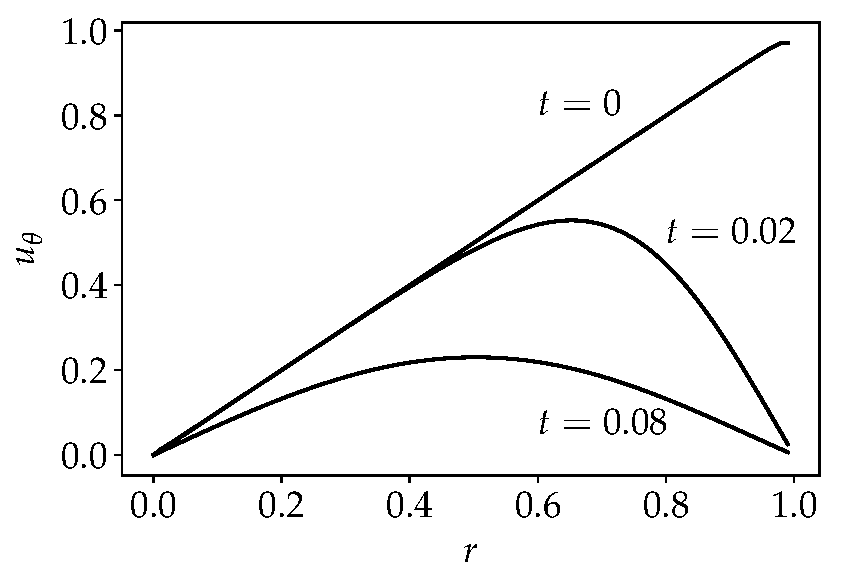
\includegraphics[width=0.7\linewidth]{Figures/Chapter2/fig_spin_vel}
\caption{The spin down of fluid initially rotating like a solid body at three different times.}
\label{fig_spin_vel}
\end{figure}


% SUBSECTION - THE LINE VORTEX

\subsection{The Line Vortex}
\label{sec_line_vortex}

Our last two examples involved fluid \emph{inside} a cylinder; let's flip that around and look at the fluid \emph{outside} a solid cylinder, rotating initially at some angular speed $\Omega$ (see Figure \ref{fig_line_setup}).  As we've done a number of times in this Chapter, we'll search first for a steady-state solution, and then look at time-dependence.

\begin{figure}
\centering
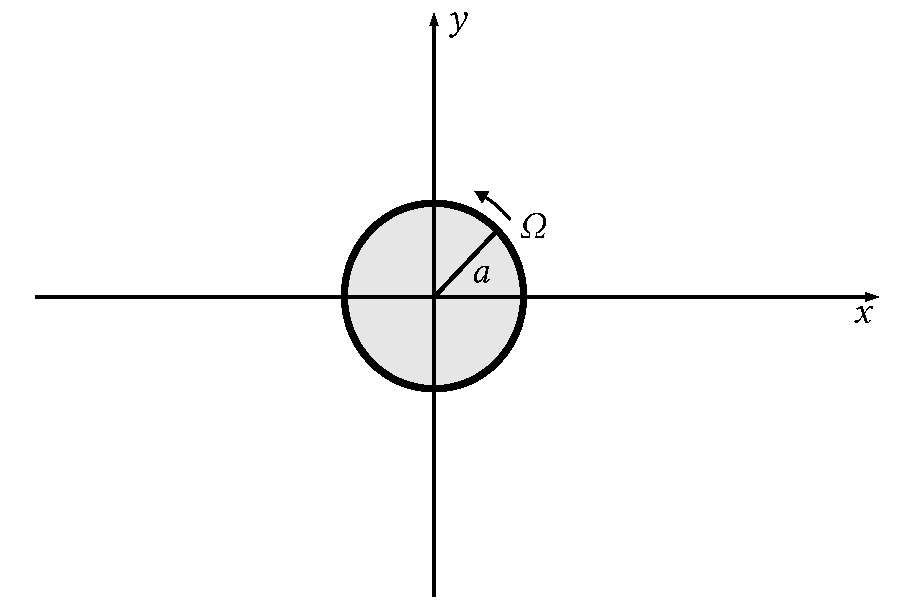
\includegraphics[width=0.7\linewidth]{Figures/Chapter2/fig_line_setup}
\caption{A solid cylinder rotating in a fluid.}
\label{fig_line_setup}
\end{figure}

We once again have circular flow, and the steady-state is described by Equation \ref{eq_spin_diffeq} and its general solution, Equation \ref{eq_cyl_steady_gen_sol},
\[
u_\theta (r) = Ar + \frac{B}{r}.
\]
Although the boundary condition is \emph{also} the same -- that $u_\theta(a) = \Omega a$ -- the difference here comes from keeping the fluid velocity finite.  Since the fluid extends out to infinity, we set $A = 0$; since there's no fluid at $r=0$, the second term won't be a problem.  Fitting the boundary condition leads to our answer,
\[
u_\theta(r) = \frac{\Omega a^2}{r}.
\]

We've seen this kind of flow before -- it's the line vortex from Example \ref{ex_vorticity_line_vortex}, with $k=\Omega a^2$.  In fact, it's customary to write this flow as
\begin{equation}
\label{eq_line_vortex}
u_\theta(r) = \frac{\Gamma_0}{2\pi r},
\end{equation}
where the constant $\Gamma_0$ is called the \emph{circulation}.  We'll explore the concept of circulation more in Chapter \ref{chap_complex_pot}.

Now let's take the cylinder away.  But we'll do it carefully -- we'll let $a \to 0$ at $t=0$, and the radius will shrink to zero instantaneously (kind of like how the boundary started moving in Section \ref{sec_imp}).  That means Equation \ref{eq_line_vortex} will give us the initial conditions, but now the evolution of the system is governed by Equation \ref{eq_ns_evol},
\[
\dfdx{u_\theta}{t} =  \nu \left( \ddfdx{u_\theta}{r} + \frac{1}{r} \dfdx{u_\theta}{r} - \frac{u_\theta}{r^2} \right).
\]

Before we solve this, I want to make a small change to this differential equation.  Let's define a new variable,
\begin{equation}
\Gamma (r, t) = 2\pi r u_\theta(r, t).
\end{equation}
Then, with a bit of work, the evolution equation becomes slightly simpler,
\begin{equation}
\label{eq_evol_gamma}
\dfdx{\Gamma}{t} = \nu \left( \ddfdx{\Gamma}{r} - \frac{1}{r} \dfdx{\Gamma}{r} \right),
\end{equation}
and the initial conditions are now given by
\begin{equation}
\Gamma(r, 0) = \Gamma_0.
\end{equation}

What about the boundary conditions?  Well, as usual we want the flow to be finite everywhere for $t>0$ (careful -- right \emph{at} $t=0$ the flow $u_\theta$ is in fact infinite, a point we'll discuss in the next section).  With our definition of $\Gamma$, that means we need
\begin{equation}
\Gamma(0, t) = 0 \quad \text{for } t>0.
\end{equation}

Now we're ready to solve this problem.  Note that it's actually \emph{scale-free} -- there's nothing here (once the cylinder disappears) to provide any physical scale.  That suggests we can seek a self-similar solution. As we did before in Section \ref{sec_self_similar}, we can define a new dimensionless variable,
\begin{equation}
\eta = \frac{r}{\sqrt{\nu t}},
\end{equation}
and assume that the solution is some function a $\eta$ alone,
\[
\Gamma(r, t) = f(\eta).
\]
I'll let you plug this into Equation \ref{eq_evol_gamma} and find the similarity solution yourself (Problem \ref{prob_sim}).  The answer is
\[
\Gamma(r, t) = \Gamma_0 \left(1 - e^{-r^2 / 4\nu t} \right),
\]
so that the fluid velocity is
\begin{equation}
\label{eq_line_vortex_vel}
u_\theta(r, t) = \frac{\Gamma_0}{2\pi r} \left( 1- e^{-r^2 / 4 \nu t} \right).
\end{equation}

Let's explore this solution a bit.  I've plotted the velocity in Figure \ref{fig_line_vortex} for a couple of different times so you can see how the speed decays.  For large radii, $r \gg \sqrt{4\nu t}$, we can drop the exponential term in Equation \ref{eq_line_vortex_vel}, and the behaviour far from the origin still looks like a line vortex:
\[
u_\theta \approx \frac{\Gamma_0}{2\pi r}.
\]
However, at small radii, $r \ll \sqrt{4 \nu t}$, we can expand the exponential and, keeping only the first two terms, get
\[
u_\theta \approx \left( \frac{\Gamma_0}{8 \pi \nu t} \right) r.
\]
This looks like solid body rotation again, with $u_\theta \propto r$.  Thus, at small radii, the flow is completely different; it's undergoes solid body rotation and has \emph{vorticity}.  It's the role of vorticity we need to discuss next.

\begin{figure}
\centering
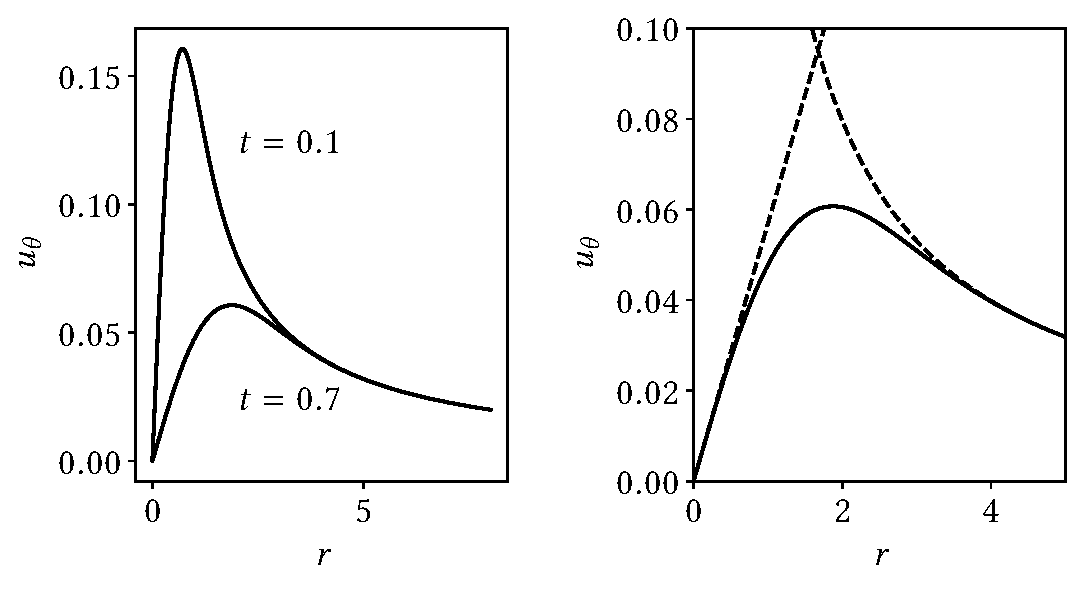
\includegraphics[width=0.8\linewidth]{Figures/Chapter2/fig_line_vortex}
\caption{The decay of a line vortex.  On the left plot, the fluid velocity is shown at two different times.  On the right plot, just $t=0.7$ is shown, along with the small- and large- radii behaviour shown as dashed lines.}
\label{fig_line_vortex}
\end{figure}

%
% --- SECTION - VISCOUS DECAY ---
% 

\section{Transport of Vorticity}

So far, all we've done is solve the Navier-Stokes equations for a variety of different situations.  Actually, the variety hasn't been all that great -- we've really only covered two kinds of flow, \emph{plane parallel shear flow} and \emph{circular flow}.  In both cases, the flow direction is parallel to the flow dependence; in the case of plane parallel shear flow, we had the fluid moving in the $x$ direction, but the speed changed along the $y$ direction only.  For circular flow, the fluid flowed in the $\theta$ direction but all dependence was along the radius $r$.  

For flows of this type, the second term in the acceleration (Equation \ref{eq_accel}) -- the so-called convective term -- is zero:
\[
(\mathbf{u} \cdot \boldsymbol{\nabla}) \uu = 0.
\]
This not only makes the Navier-Stokes equations significantly easier (it eliminates their nonlinear nature, for example), it also allows for only one kind of \emph{vorticity transport} as we'll see in a moment.

First, though, let's go back and take a look at two of our results:  the impulsively moved boundary in Section \ref{sec_self_similar} and the line vortex decay in Section \ref{sec_line_vortex}.  Both of these examples illustrated an interesting aspect concerning vorticity.  For the impulsively moved boundary, the vorticity is (see Problem \ref{prob_vorticity})
\begin{equation}
\label{eq_vort_1}
\omega = \frac{U}{\sqrt{\pi \nu t}} \, e^{-y^2 / 4 \nu t}.
\end{equation}
As $t \to 0$, the vorticity becomes infinite at the boundary $y=0$ but is zero everywhere else -- this is called a \emph{vortex sheet}.  The line vortex is similar, with 
\begin{equation}
\label{eq_vort_2}
\omega = \frac{\Gamma_0}{4\pi \nu t} \, e^{-r^2 / 4 \nu t}.
\end{equation}
This time, as $t \to 0$, the vorticity becomes infinite along $r=0$, but zero elsewhere, so this is a \emph{vortex line}.  Figure \ref{fig_vorticity_transport} shows the two vorticities at various times.  As you can see, the vorticity is strongly concentrated at either $y=0$ or $r=0$ at early times, but then becomes more ``spread out'' as time progresses.  It's this process of \emph{vorticity diffusion} that I want to discuss.

\begin{figure}
\centering
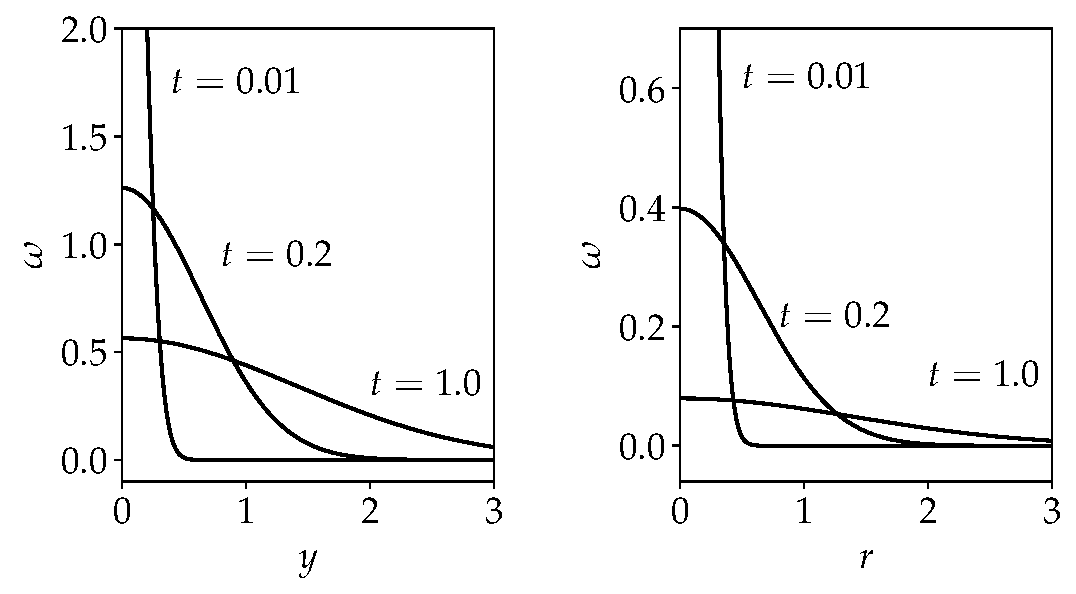
\includegraphics[width=0.8\linewidth]{Figures/Chapter2/fig_vorticity_transport}
\caption{The vorticity $\omega$ at a few different times for the impulsively moved boundary (left) and the line vortex (right).  In both cases an infinite amount of vorticity concentrated at one point spreads throughout the fluid.}
\label{fig_vorticity_transport}
\end{figure}

In fact, there are two different ways that vorticity can change in a fluid.  We can see this by taking the curl of both sides of the Navier-Stokes equations to get
\begin{equation}
\dfdx{\vort}{t} + (\uu \cdot \grad) \vort = (\vort \cdot \grad) \uu + \nu \nabla^2 \vort
\end{equation}
(this isn't exactly straightforward to derive, but we'll deal with it later in Section \ref{sec_vorticity_eq} for ideal fluids, and for now I don't want any distractions).  In two dimensional flow, like we've been dealing with in this Chapter, it becomes a little simpler, since the first term on the right hand side will becomes zero -- the vector $\vort$ will point in the $z$ direction, so the term $\vort \cdot \grad)$ will have only a $z$ derivative acting on $\uu$, which of course only depends on $x$ and $y$.  That means this vorticity equation looks like
\[
\dfdx{\omega}{t} + (\uu  \cdot \grad) \omega = \nu \left( \ddfdx{\omega}{x} + \ddfdx{\omega}{y} \right).
\]
We can now highlight the two ways that the vorticity can change:  first by viscous \emph{diffusion}, handled by the term with the viscosity in it, and second by \emph{convection}, which is the second term on the left.  By convection, I simply mean that the vorticity is transported through the fluid by the individual fluid elements themselves; in cases where the viscosity is zero, this is the only way to transport vorticity, and in that case each fluid element conserves its vorticity.

In all of the examples we've done so far, this convection term is zero, just like the convective acceleration is zero.  That means the vorticity is only transported through the fluid by diffusion.  In general, both mechanisms are at work, but of course those situations are significantly more difficult to deal with.  One example that's actually solvable -- with some difficulty and some numerical work -- is detailed in Section \ref{sec_boundary_layers}.

%
% --- SECTION - ADVANCED TOPIC 1 ---
% 

\section{Advanced Topics 1: Deriving the Navier-Stokes Equations}
\label{sec_ns_deriv}

%
% --- SECTION - ADVANCED TOPIC 2 ---
% 

\section{Advanced Topics 2: Boundary Layers}
\label{sec_boundary_layers}

The presence of a boundary layer in a fluid is one of the big differences between viscous flow and inviscid.  To explore boundary layers further, let's set up a fairly simple situation.  Consider fluid in the region $y \ge 0$, above a rigid boundary along $y=0$.  Suppose the flow is given by
\begin{equation}
\mathbf{u} = [\alpha x, -\alpha y, 0],
\end{equation}
where $\alpha$ is some constant.  We've seen this type of flow before, in Chapter 1 -- it's the flow about a stagnation point.  The streamlines are shown in Figure \ref{fig_boundary_stream}.

\begin{figure}
\centering
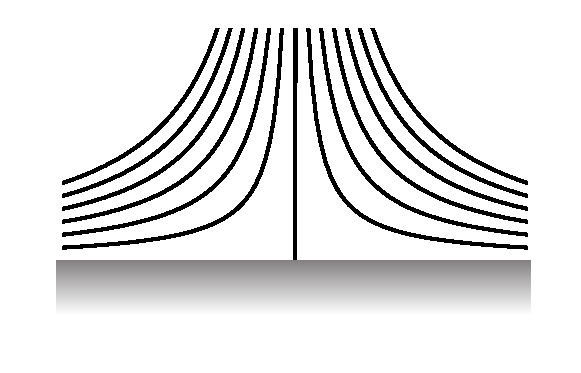
\includegraphics[width=0.6\linewidth]{Figures/Chapter2/fig_boundary_stream}
\caption{Streamlines for flow about a stagnation point.  The fluid lies above the $x$-axis.}
\label{fig_boundary_stream}
\end{figure}


Now, this flow satisfies the Navier-Stokes equation, with a pressure given by
\begin{equation}
\label{eq_boundary_pressure}
p(x, y) = -\frac{1}{2} \rho \alpha^2 ( x^2 + y^2) + \text{ constant}.
\end{equation}
However, it \emph{doesn't} satisfy the no-slip boundary condition -- the fluid velocity isn't zero at the boundary!  This is actually fine if we're dealing with an inviscid fluid, where we expect the flow to be directed along the boundary, but doesn't work for a viscous fluid.  It also has no indications of a boundary layer.

We need to fix things up, then, to account for the boundary layer and viscosity.  We can do that by changing our flow slightly to
\begin{equation}
\label{eq_boundary_trial}
\mathbf{u} = [\alpha x f'(\eta), -\sqrt{\nu \alpha} f(\eta), 0],
\end{equation}
where
\[
\eta = \sqrt{ \frac{\alpha}{\nu}} y
\]
is a dimensionless length parameter.  Here, the function $f(\eta)$ is an unknown function that we'll solve for shortly; notice that if $f(\eta) = \eta$, we get back our original flow about a stagnation point.  However, in order to satisfy the no-slip condition and get zero velocity at $y=0$, we need $f \to 0$ \emph{and} $f' \to 0$ when $\eta \to 0$.  Clearly $f(\eta) = \eta$ won't do the trick.  On the other hand, we do expect the flow far away from the boundary to look like our original stagnation point flow; we'll return to this later.

To find the function $f(\eta)$ properly, then, we need to make sure that this flow still satisfies the Navier-Stokes equation.  If we plug in the velocity in Equation (\ref{eq_boundary_trial}) into the Navier-Stokes equation, the $x$ and $z$ equations become
\begin{equation}
\label{eq_boundary_ns1}
\alpha^2 x f'^2 - \alpha^2 x f f'' = -\frac{1}{\rho} \frac{\partial p}{\partial x} + \alpha^2 x f'''
\end{equation}
and
\begin{equation}
\sqrt{\alpha^3 \nu } ff' = \frac{1}{\rho} \frac{\partial p}{\partial y} - \sqrt{\alpha^3 \nu} f'',
\end{equation}
respectively.  Let's rearrange the second equation slightly to get
\[
-\frac{1}{\sqrt{\alpha^3 \nu}} \frac{1}{\rho} \frac{\partial p}{\partial y} = \frac{1}{2} \frac{d}{d\eta} f^2 + \frac{d}{d\eta} f'.
\]
We can then replace the $\partial y$ derivative with $\partial \eta$, since
\[
\frac{d\eta}{dy} = \sqrt{\frac{\alpha}{\nu}},
\]
to get
\[
-\frac{1}{\alpha \nu \rho} \frac{\partial p}{\partial \eta} = \frac{1}{2} \frac{d}{d\eta} f^2 + \frac{d}{d\eta} f'.
\]
Finally, integrate with respect to $\eta$:
\[
-\frac{1}{\alpha \nu \rho} p = \frac{1}{2} f^2 + f' + g(x),
\]
where $g(x)$ is the integration ``constant.''  This is a useful result:  if we now take the derivative with respect to $x$, we can see that 
\[
\frac{\partial p}{\partial x} \propto \frac{\partial g}{\partial x}.
\]
In other words, $\partial p / \partial x$ is at best a function of $x$.

We can now return to the other Navier-Stokes equation, Equation (\ref{eq_boundary_ns1}), and separate variables so that all $x$ terms are on one side and all $\eta$ terms are on the other:
\[
-\frac{1}{\alpha^2 \rho x} \frac{\partial p}{\partial x} = f'^2 - ff'' - f'''.
\]
Since $x$ and $\eta$ (which is really just $y$) are independent, each side of this equation must be a constant.  What is the value of that constant?  To find it, we'll compare with the inviscid solution for the pressure, Equation (\ref{eq_boundary_pressure}).  To have our pressures agree, we need the constant to be one.

Finally, then, we have our last equation we need to solve,
\begin{equation}
f''' + ff'' - f'^2 + 1 = 0.
\end{equation}
As we've discussed above, the boundary conditions are
\[
f(0) = 0; \quad f'(0) = 0; \quad \text{and} \quad f'(\infty) = 1,
\]
where the last condition ensure that we return to our original flow (with $f(\eta) = \eta$) far away from the boundary.

This equation must be solved numerically, but it can be tricky to do so while making sure the boundary conditions match.  Code to do it is provided, and the results are shown in Figures \ref{fig_boundary_result1} and \ref{fig_boundary_result2}.  As you can see, there is now a small boundary layer where the velocity drops to zero, but away from the boundary the flow is indistinguishable from the inviscid case.  Despite the complexity of this example, it's a good one for exploring exactly how the boundary layer develops for viscous flows.

\begin{figure}
\centering
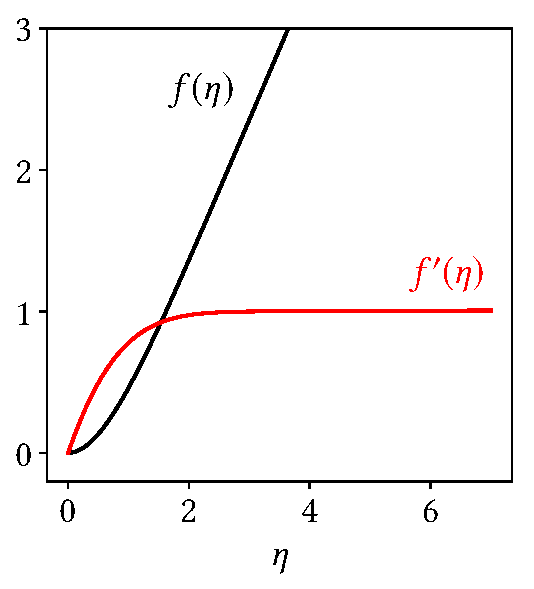
\includegraphics[width=0.4\linewidth]{Figures/Chapter2/fig_boundary_result1}
\caption{The function $f(\eta)$ (black) and $f'(\eta)$ (red).  Note that the boundary layer is clear -- it extends out to around $\eta \sim 2$.  After that, $f(\eta) \approx \eta$.}
\label{fig_boundary_result1}
\end{figure}

\begin{figure}
\centering
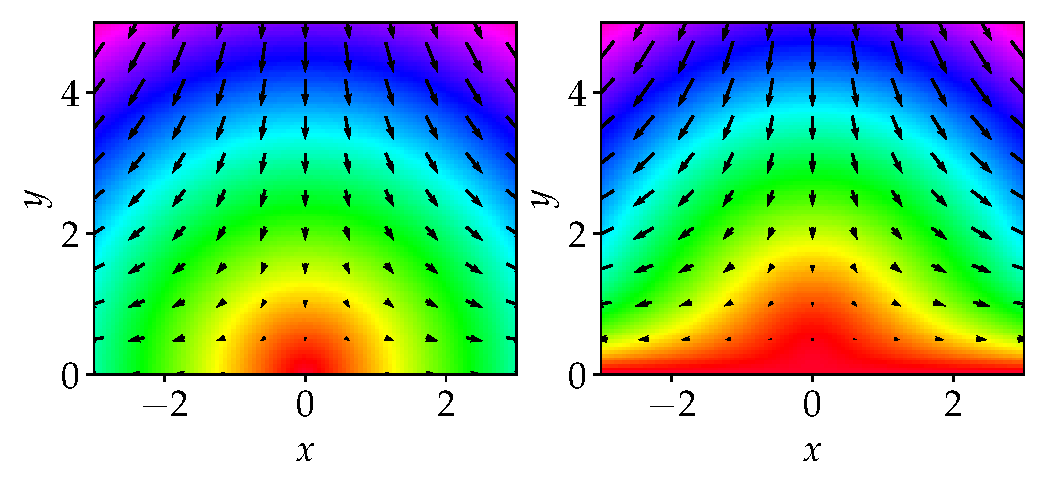
\includegraphics[width=0.9\linewidth]{Figures/Chapter2/fig_boundary_result2}
\caption{Vector plots of the invisid flow (left) and viscous flow (right).  The boundary layer can be clearly seen in the flow -- the red area indicates small velocity.}
\label{fig_boundary_result2}
\end{figure}


\section*{Problems}
\addcontentsline{toc}{section}{Problems}


\begin{problem}[Poiseuille flow with gravity]
\label{prob_poise_grav}
In Section \ref{sec_poise_1d} we examined Poiseuille flow in one dimension, but without the force of gravity playing a role.  Repeat our work to find the fluid velocity and pressure in the fluid, but this time include gravity in (a) the $z$ direction (so $\mathbf{g} = [0,0,g]$) and (b) the $x$ direction (so $\mathbf{g} = [g, 0, 0]$).  Comment on how, if at all, the velocity changes.
\end{problem}

\begin{problem}[Flow down an incline]
Suppose fluid has been flowing down an inclined plane for a long time, as shown in Figure \ref{fig_incline_setup}.  The fluid has a height $h$ above the plane, and above the fluid is air.  Gravity points straight down as shown.  What is the pressure abd velocity of the fluid?  

\emph{Hint:} One of the boundary conditions is obvious, but the second is trickier.  Assume the pressure at the surface of the fluid is at atmospheric pressure, and also that there is no tangential stress across the surface (otherwise it wouldn't be a stable surface); see Equation \ref{eq_visc_def}.
\end{problem}

\begin{figure}
\centering
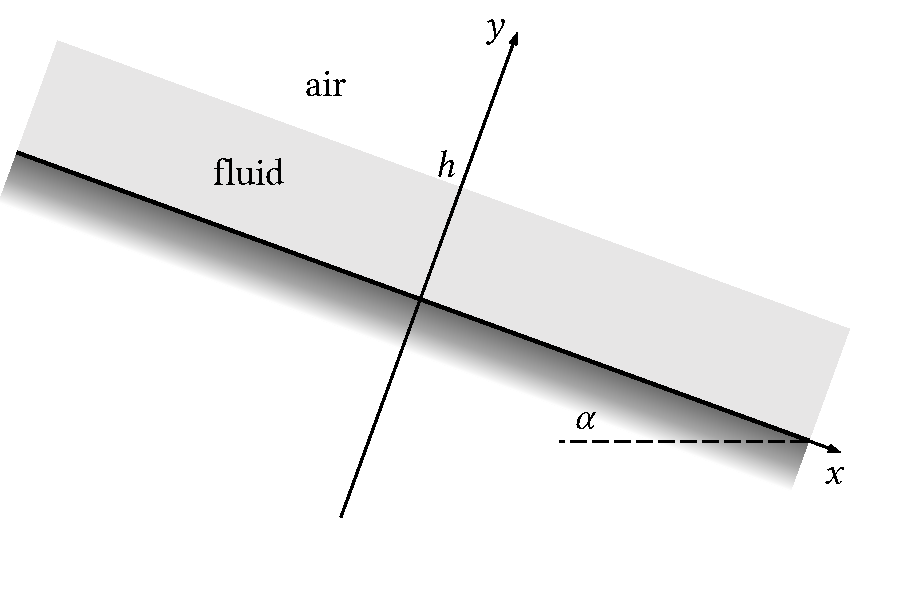
\includegraphics[width=0.7\linewidth]{Figures/Chapter2/fig_incline_setup}
\caption{Fluid flows down an incline.}
\label{fig_incline_setup}
\end{figure}

\begin{problem}[Poiseuille flow in two dimensions]
\label{prob_poise_2d}
Consider the rectangular pipe shown in Figure \ref{fig_poise_2d_setup}.  Suppose fluid flows down the $x$-axis thanks to a constant pressure gradient 
\[
\frac{dp}{dx} = -P,
\]
just as in the Poiseuille problem we discussed in Section \ref{sec_poise_1d}.  Find the velocity of the fluid within the pipe, and think about how to best visualize the flow.  

\emph{Hint:} The flow will now depend on $z$ as well as $y$, and the differential equation will be nonhomogeneous, so you'll have to figure out a way to \emph{make} it homogeneous.  Think about the 1D solution we did earlier.  This is a lengthy, difficult problem, so here's the final answer:
\[
u(y, z) =  \frac{P}{2\nu \rho} \left[ (ay - y^2) + \frac{8a^2}{\pi^3} \sum_{n=1,3,5, \dots} \frac{1}{n^3} \frac{1}{\cosh (n\pi b / 2a)} \sin (n\pi y / a) \cosh(n \pi z / a) \right].
\]
\end{problem}

\begin{figure}
\centering
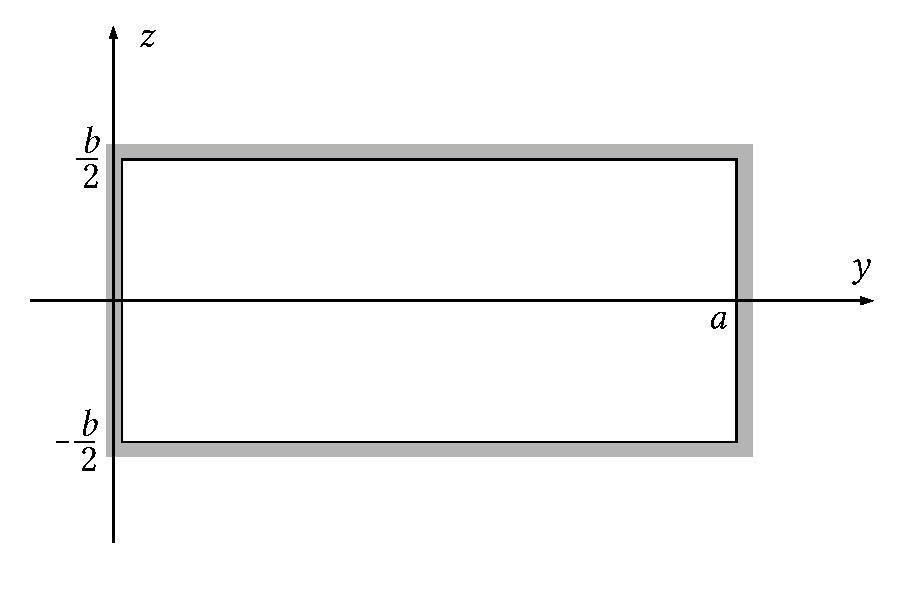
\includegraphics[width=0.7\linewidth]{Figures/Chapter2/fig_poise_2d_setup}
\caption{Fluid flows through a rectangular pipe.}
\label{fig_poise_2d_setup}
\end{figure}


\begin{problem}[Poiseuille flow in a cylinder]
\label{prob_poise_cyl}
The physician Poiseuille originally studied the problem of blood flowing through blood vessels. We can model that with a Newtonian fluid flowing down a pipe of circular cross-section (radius $a$).  If the pumping of the heart provides a constant pressure gradient within the blood vessel of $dp/dz = -P$,  find the velocity of the fluid.  Plot the velocity as a function of radius.
\end{problem}

\begin{problem}[Starting up Poiseuille flow]
\label{prob_poise_time}
For one last Poiseuille flow problem, consider the 1D example of Section \ref{sec_poise_1d} again.  This time, however, suppose that the fluid in the channel is at rest initially.  At time $t = 0$, the pressure gradient $dp/dx = -P$ starts instantaneously.  How does the fluid respond?  Find the velocity as a function of time, and plot it for a few different times.  What does the flow look like for $t \gg h^2 / \nu$?
\end{problem}

\begin{problem}[Fluid above an oscillating floor]
\label{prob_cyl_osc}
Fluid lies above an infinitely rigid plane at $y=0$.  The plane is oscillating back and forth along the $x$-direction with velocity
\[
u_\text{plane} = U \cos \omega t.
\]
Find the velocity of the fluid,\footnote{This is Stokes' second problem.} and plot it at some time $t$.  How far above the plane does the oscillatory motion seem to affect the fluid?

\emph{Hint:}  Try a solution of the form $f(y) e^{i \omega t}$ and take the real part at the end.
\end{problem}

\begin{problem}[The incompressibility condition for circular flow]
\label{prob_cyl_incomp}
Show that the incompressibility condition is automatically satisfied of the flow is if the form 
\[
\mathbf{u} = u_\theta (r, t) \, \hat{\theta}.
\]
\end{problem}

\begin{problem}[Fluid between two cylinders]
\label{prob_cyl_two}
Fluid lies between two concentric cylinders.  The inner solid cylinder, of radius $a$, rotates with angular velocity $\Omega_a$, and the outer hollow cylinder, of radius $b$, rotates with angular velocity $\Omega_b$.  Assuming the flow is steady, find the velocity of the fluid.
\end{problem}

\begin{problem}[Similarity solution examined]
\label{prob_sim}
Consider the decay of a line vortex, which we looked at in Section \ref{sec_line_vortex}.  The evolution of the vortex is given by Equation (\ref{eq_evol_gamma}).  Solve this equation for $\Gamma(r, t)$ by assuming a similarity solution of the form
\[
\Gamma(r, t) = f(\eta),
\]
where 
\[
\eta = \frac{r}{\sqrt{\nu t}},
\]
and show that the velocity is given by Equation (\ref{eq_line_vortex_vel}).  Plot the circulation $\Gamma(r, t)$ at two different times; scale your axis appropriately to show that the curve is self-similar.
\end{problem}

\begin{problem}[Flow with a spinning bottom]
\label{prob_spin_bottom}
Suppose that viscous fluid occupies the region between two rigid plane boundaries at $z = 0$ and $z = h$.  The upper boundary is at rest, but the lower boundary rotates with constant angular speed $\Omega$ about the $z$-axis.  Assume the flow is steady.  (This is a simplistic model for a blender -- at least the mixing part of it.)

(a) Argue that, on physical grounds, you'd expect a solution of the form
\[
\mathbf{u} = u_\theta (r, z) \, \hat{\theta}.
\]
What are the boundary conditions for the flow?

(b) But there's a problem with that form of the flow.  Use the cylindrical form of the Navier-Stokes equations to show that, assuming flow of the form above, 
\[
u_\theta = \sqrt{\frac{r}{\rho} \frac{\partial p}{\partial r} }.
\]
Furthermore, show that $p$ doesn't depend on $z$.  Thus, argue that $u_\theta = u_\theta(r)$ only.  Is this form of the flow compatible with the boundary conditions?  Therefore, despite your reasoning above, we need a \emph{secondary flow} along either $r$ or $z$ (or both).  

(So, going back to the blender model, this is why when I make a smoothie in the morning, there is clearly flow along the $\hat{r}$ and $\hat{z}$ directions.  Look for it yourself next time you make a smoothie!)
\end{problem}

\begin{problem}[Vorticity of simple flows]
\label{prob_vorticity}

(a) Find the vorticity of the fluid in the impulsively moved single plate example (Section \ref{sec_self_similar}) and show that it is given by Equation (\ref{eq_vort_1}).

(b) Find the vorticity of the fluid in the line vortex example (Section \ref{sec_line_vortex}) and show that it is given by Equation (\ref{eq_vort_2}).
\end{problem}



\chapter{Ideal Fluids}

We'll start our exploration of solutions to the Navier-Stokes equation with \emph{ideal fluids}, which we'll define as 
\begin{enumerate}
\item having no viscosity, and
\item having constant density (incompressible).
\end{enumerate}
Of course, \emph{real} fluids always have \emph{some} viscosity; however, as discussed in Section \ref{sec_viscosity}, in some cases an ideal fluid can be a good approximation to a real one.  Keep in mind, however, that the boundary layer present in viscous fluids can never be described by an ideal fluid, so we'll miss some of the physics due to that.

Under these assumptions, the Navier-Stokes equation is usually called \emph{Euler's equation},
\begin{equation}
\label{eq_euler}
\boxed{
\frac{D \uu}{Dt} = -\frac{1}{\rho} \grad p + \mathbf{g}.
}
\end{equation}
The incompressibility condition,
\begin{equation}
\div \uu = 0,
\end{equation}
remains the same.





\section{Static Fluids}

The simplest solution to either the Navier-Stokes equation or Euler's equation is the trivial one:  suppose the fluid is at rest, so that $\uu = 0$ everywhere.  Then Euler's equation reduces to 
\[
0 = -\frac{1}{\rho} \grad p + \mathbf{g},
\]
or 
\[
\grad p = \rho \mathbf{g}.
\]
If we take the direction of gravity to be down, so that $\mathbf{g} = [0,0,-g]$, this equation says
\[
\frac{\partial p}{\partial x} = 0, \quad \frac{\partial p}{\partial y} = 0, \quad \frac{\partial p}{\partial z} = -\rho g.
\]
The first two equations just say that the pressure $p$ doesn't depend explicitly on $x$ or $y$, and we can integrate the third to get
\begin{equation}
p = p_0 - \rho g z,
\end{equation}
where $p_0$ is the integration constant.  If our fluid has a ``free surface'' -- it's open to the atmosphere -- at $z=0$, then $p_0$ is the atmospheric pressure.

This result is simple and tells us what we pretty much know:  as you go down in depth ($z < 0$) in a fluid, the pressure increases.  Note, however, that we've assumed the density $\rho$ stays constant; in some fluids (like the atmosphere) it's a bad assumption, while in others (like the ocean, at least for reasonable depths) it's okay.






\section{Bernoulli's Principle}

For our next result, we'll first need to rewrite Euler's equation.  Since gravity is a conservative force, we can always write it in terms of the gradient of a scalar, so that
\[
\mathbf{g} = - \grad \chi,
\]
where $\chi$ is the gravitational potential.  For example, setting $\chi = gz$ gives us our usual $\mathbf{g}$ pointing down along the $z$ axis.

With this change, Euler's equation becomes
\[
\frac{\partial \uu}{\partial t} + (\uu \cdot \grad) \uu = -\grad \left( \frac{p}{\rho} + \chi \right).
\]
It turns out that the second term on the left can be written as (see Problem \ref{prob_vc3})
\begin{equation}
 (\uu \cdot \grad) \uu = (\curl \uu ) \times \uu + \grad (\tfrac{1}{2} \uu^2).
\end{equation}
Note that I've written $\uu^2$ for $\uu \cdot \uu$; as usual, be careful of all the different $u$'s we deal with.  With this substitution, and moving the gradient onto the right hand side, Euler's equation is now
\begin{equation}
\frac{\partial \uu}{\partial t} + (\curl \uu ) \times \uu = -\grad \left( \frac{p}{\rho} + \tfrac{1}{2} \uu^2 + \chi \right).
\end{equation}

This doesn't look any better than the original form of Euler's equation, though.  We can clean it up a bit by defining
\[
H \equiv \frac{p}{\rho} + \tfrac{1}{2} \uu^2 + \chi,
\]
which is sometimes called the ``total head'' or ``energy head'' of the flow.  If we also assume the flow is \emph{steady}, we then have
\begin{equation}
(\curl \uu ) \times \uu = -\grad H.
\label{eq_bernoulli}
\end{equation}
One last step -- take the dot product with $\uu$ for both sides:
\[
\uu \cdot [(\curl \uu ) \times \uu] = -\uu \cdot \grad H.
\]
But now the left hand side is zero -- the term in the square brackets has a direction perpendicular to $\uu$, so the dot product with $\uu$ vanishes.  

So we're left, finally, with Bernoulli's streamline theorem, which says that, for steady flow,
\begin{equation}
\boxed{
(\uu \cdot \grad) H  = 0.
}
\end{equation}
This means that $H$ is \emph{constant along a streamline} for steady flow.

If the fluid is also irrotational, so that $\curl \uu = 0$, equation (\ref{eq_bernoulli}) gives us the stronger statement
\begin{equation}
\boxed{
\grad H = 0,
}
\end{equation}
so that $H$ is constant everywhere in the fluid.

\begin{example}[A leaky bucket]
A large tank of water, open to the atmosphere at the top, suddenly springs a leak near the bottom (see Figure \ref{fig_leaky_bucket}).  If the hole is 1.0 m below the free surface, what is the speed of the water as it comes out the hole?

\begin{figure}
\centering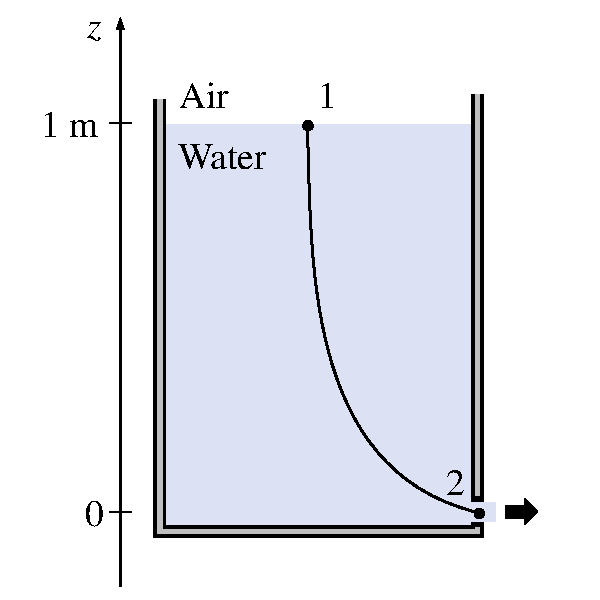
\includegraphics[width=0.5\linewidth]{Figures/Chapter3/fig_leaky_bucket}
\caption{A large tank of water has sprung a leak.  How fast is the water moving as it comes out of the hole?}
\label{fig_leaky_bucket}
\end{figure}


This is a good case for Bernoulli's principle, since the flow is (approximately) steady -- the surface will drop only slowly if the hole is small.  We can therefore use the streamline theorem:
\[
H = \frac{p}{\rho} + \tfrac{1}{2} \uu^2 + gz = \text{constant}.
\]
Presumably there exists a streamline that connects the free surface at the top of the tank with the hole (joining points 1 and 2 as shown in Figure \ref{fig_leaky_bucket}).  Then we can evaluate $H$ at both points:
\begin{itemize}
\item Point 1 $\to H_1 = \frac{p_1}{\rho} + \tfrac{1}{2} \uu_1^2 + gz_1$
\item Point 2 $\to H_2 = \frac{p_2}{\rho} + \tfrac{1}{2} \uu_2^2 + gz_2$
\end{itemize}
But $p_1 = p_2 = p_0$ since both locations are open to the atmosphere.  We'll also take $\uu_1 = 0$, since the surface drops only very slowly.  Finally, using the coordinate system shown in Figure \ref{fig_leaky_bucket}, we have $z_2 = 0$ (and $z_1 = 1$ m).

Setting $H_1 = H_2$ then gives us
\[
\frac{p_0}{\rho} + gz_1 = \frac{p_0}{\rho} + \tfrac{1}{2} \uu_2^2.
\]
The pressure terms cancel, and we can rearrange for the speed of the water:
\[
|\uu| = \sqrt{2gz_1} \approx 4.4 \text{ m/s}.
\]
\end{example}









\section{The Vorticity Equation}
\label{sec_vorticity_eq}

Let's rewrite Euler's equation again, this time in terms of the vorticity.  Going back to equation (\ref{eq_bernoulli}) and writing $\vort = \curl \uu$, we have
\[
\frac{\partial \uu}{\partial t} + \vort \times \uu = -\grad H.
\]
Take the curl of both sides:
\[
\frac{\partial \vort}{\partial t} + \curl (\vort \times \uu) = -\curl \grad H.
\]
But the curl of a gradient is identically zero (see Problem \ref{prob_vc2}), so the right hand side vanishes.

Now, there's a vector identity (another one!) that says, for two vectors $\mathbf{F}$ and $\mathbf{G}$, that
\begin{equation}
\curl (\mathbf{F} \times \mathbf{G}) = (\mathbf{G} \cdot \grad) \mathbf{F} - (\mathbf{F} \cdot \grad) \mathbf{G} + \mathbf{F} (\div \mathbf{G}) - \mathbf{G} (\div \mathbf{F})
\end{equation}
(see Problem \ref{prob_vc4}).  Using this in the equation above, with $\mathbf{F} \to \vort$ and $\mathbf{G} \to \uu$, gives us
\[
\frac{\partial \vort}{\partial t} + (\uu \cdot \grad) \vort - (\vort \cdot \grad)\uu + \vort (\div \uu) - \uu(\div \vort) = 0.
\]
Of course, we're dealing with an ideal fluid, so $\div \uu = 0$, and, since $\vort$ is a curl, $\div \vort = 0$ identically (see Problem \ref{prob_vc2} again for that one).  So the fourth and fifth terms vanish, and we have
\[
\frac{\partial \vort}{\partial t} + (\uu \cdot \grad) \vort = (\vort \cdot \grad)\uu.
\]
Finally, we can combine the two terms on the right hand side -- that's the definition of the material derivative of $\vort$ -- and we have, at long last, the \emph{vorticity equation},
\begin{equation}
\label{eq_vorticity}
\boxed{
\frac{D \vort}{Dt} = (\vort \cdot \grad) \uu.
}
\end{equation}

This equation will prove useful every once in a while for us.  In particular, for a two dimensional flow, where 
\[
\vort = (0,0,\omega),
\]
it's easy to see that the right hand side becomes zero, and 
\begin{equation}
\frac{D \vort}{Dt} = 0.
\end{equation}
This means that the vorticity of each individual fluid element is conserved, a result we'll use later.  Furthermore, if the flow is also steady, this becomes
\begin{equation}
(\uu \cdot \grad) \omega = 0,
\end{equation}
and the vorticity is constant along streamlines in this case.







\section{Example: Uniformly Rotating Fluid}

A classic problem with ideal fluids is the spinning water bucket example.  In short, we'll fill a bucket with water and start rotating the bucket.  Eventually, the water will start rotating as well and will eventually come to a steady state, with velocity
\begin{equation}
\label{eq_bucket_vel}
\uu = [-\Omega y, \Omega x, 0],
\end{equation}
where we've oriented our coordinates so that the $z$-axis runs up the symmetry axis of the bucket -- in other words, the rotation is about the $z$-axis.

By the way, you might be wondering where this velocity comes from.  After all, we didn't solve Euler's equation to get it; in fact, the fluid would require \emph{viscosity} to get spun up like this, so Euler's equation wouldn't even work to describe the spin-up.  However, once the fluid is rotating, Euler will suffice to examine the system.  Incidentally, we'll do the viscous problem later, and you'll see how a rotating boundary will indeed spin up the fluid inside.

If you look at a good photograph of this, you'll see that the surface of the water is \emph{curved} (Fig. \ref{fig_bucket}).  What is the shape of this free surface?

\begin{figure}[t]
\centering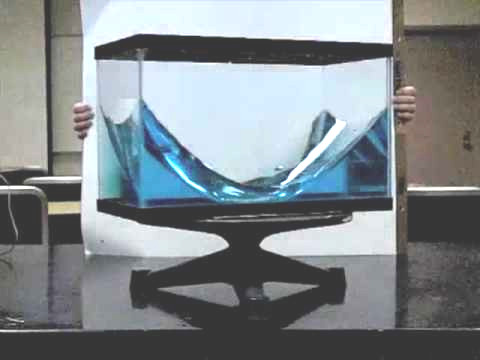
\includegraphics[width=0.5\linewidth]{Figures/Chapter3/fig_water_bucket.jpg}
\caption{A tank of water is smoothly spun up, causing the water to ``climb'' the sides of the tank.  From Dan Russell (\url{https://www.youtube.com/watch?v=Zip9ft1PgV0}).}
\label{fig_bucket}
\end{figure}

Well, the thing that all fluid elements along the free surface have in common is that they have the same pressure -- namely, since they're at the surface, atmospheric pressure $p_0$.  Let's find the pressure in the water, then.

To do that, we'll use Euler's equation, since the flow must satisfy that.  The $x$ component of equation (\ref{eq_euler}) (or the ``$u$'' component), with $\mathbf{g} = [0,0,-g]$, is
\[
\frac{\partial u}{\partial t} + u\frac{\partial u}{\partial x} +  v\frac{\partial u}{\partial y} + w\frac{\partial u}{\partial z} = -\frac{1}{\rho} \frac{\partial p}{\partial x}.
\]
But the flow is \emph{steady}, and $u$ doesn't depend on $x$ or $z$.  Substituting in the fluid velocity in equation (\ref{eq_bucket_vel}), this equation reduces to
\begin{equation}
\label{eq_px}
\frac{\partial p}{\partial x} = \rho \Omega^2 x.
\end{equation}
Similarly, the $v$ and $w$ equations reduce to
\begin{equation}
\label{eq_py}
\frac{\partial p}{\partial y} = \rho \Omega^2 y
\end{equation}
and
\begin{equation}
\label{eq_pz}
\frac{\partial p}{\partial z} = -\rho g.
\end{equation}

We can integrate to find the pressure $p(x, y, z)$.  From equation (\ref{eq_px}) we get
\[
p = \tfrac{1}{2} \rho \Omega^2 x^2 + f(y, z),
\]
where the function $f(yz)$ is there since equation (\ref{eq_px}) is a \emph{partial} derivative -- we don't just get a constant of integration, but a possible function of the other two variables.  Integrating equation (\ref{eq_py}) gives
\[
p = \tfrac{1}{2} \rho \Omega^2 y^2 + g(x, z),
\]
and integrating equation (\ref{eq_pz}) gives
\[
p = -\rho g z + h(x, y).
\]
By inspection, it's clear that the pressure must be
\[
p(x, y, z) = \tfrac{1}{2} \rho \Omega^2 (x^2 + y^2) - \rho gz + p_1,
\]
where $p_1$ is a constant -- it's the pressure at the origin.

That's the pressure everywhere in the water.  To find the shape of the free surface, we'll set $p = p_0$ and solve for the height $z$:
\begin{equation}
z = \frac{\Omega^2}{2g} (x^2 + y^2) + \left( \frac{p_1 - p_0}{\rho g} \right).
\end{equation}
This is a \emph{paraboloid} -- see Fig. \ref{fig_bucket_para} -- and it matches the shape in the photograph in Figure \ref{fig_bucket}.

\begin{figure}
\centering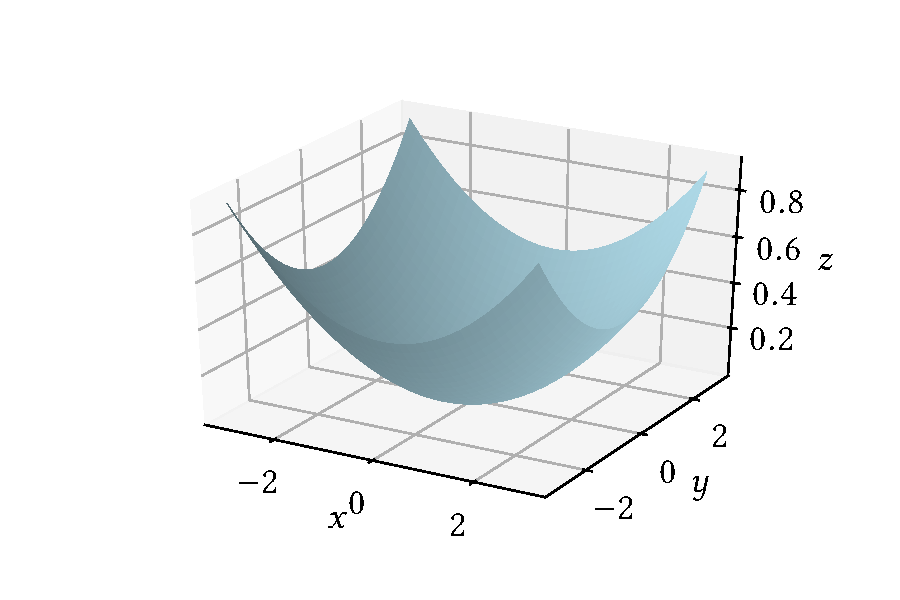
\includegraphics[width=0.8\linewidth]{Figures/Chapter3/fig_paraboloid}
\caption{The free surface of the spinning bucket problem is a paraboloid.  \href{https://nbviewer.jupyter.org/github/josephmacmillan/IntroFluidDynamics/blob/master/Jupyter/3-IdealFluids.ipynb\#Figure-3.3:--Uniformly-rotating-fluid}{[Link to code]}}
\label{fig_bucket_para}
\end{figure}





\section{The Velocity Potential and Laplace's Equation}

For any irrotational flow, where
\[
\curl \uu = 0,
\]
a scalar function $\phi$ can be defined such that
\begin{equation}
\label{eq_vel_pot}
\boxed{
\uu = \grad \phi.
}
\end{equation}
Then, since the curl of a gradient is zero, irrotationality is automatically satisfied.  Here, $\phi$ is called the \emph{velocity potential}.

Alternatively, we could write the potential as
\begin{equation}
\label{eq_vel_pot2}
\phi = \int_\mathcal{O}^\mathcal{P} \uu \cdot d\mathbf{x},
\end{equation}
where $\mathcal{O}$ is an arbitrary point in the fluid.  There's a subtle point here, though, so be careful.  As long as the region is \emph{simply connected} -- that is, the fluid has no holes in it -- the path between $\mathcal{O}$ and $\mathcal{P}$ doesn't matter, and $\phi$ will be a single-valued function.

However, if the region is \emph{multiply connected} -- it has holes, regions where there is no fluid -- the integral \emph{could} depend on the path and $\phi$ will be a multivalued function of position.  Let's do some examples to investigate this in detail.

\begin{example}[Uniform flow]
\label{ex_uniform}
Let's start with uniform flow, which is simple and one we'll use extensively. Suppose $\uu = (U, 0, 0)$, where $U$ is the constant velocity of the flow in the $x$-direction. Using either equation (\ref{eq_vel_pot}) or (\ref{eq_vel_pot2}), we can see that
\begin{equation}
\phi = Ux = U r\cos \theta.
\end{equation} 
I've written the potential down in both Cartesian coordinates and also cylindrical; we'll need the cylindrical version later on.
\end{example}

\begin{example}[Flow past a stagnation point]
Recall the flow past a stagnation point, given by
\[
\uu = (\alpha x, -\alpha y, 0).
\]
This is irrotational flow (check if you want!), and to find the velocity potential, write
\[
\frac{\partial \phi}{\partial x} = u = \alpha x \quad \text{and} \quad \frac{\partial \phi}{\partial y} = v = -\alpha y.
\]
Integrating and combining suggests
\[
\phi(x, y) = \tfrac{1}{2} \alpha (x^2 - y^2) + c,
\]
where $c$ is the integration constant.  Note, however, that the fluid velocity, as opposed to the potential, is the physically meaningful quantity; since we take a derivative to get to the velocity, we can set the constant $c$ to zero without worry that it's meaningful.

Note that here $\phi$ is a single-valued function of $x$ and $y$.  That means that, for any point in the fluid, $\phi$ has a single value.
\end{example}

\begin{example}[Line vortex flow]
For our last example, consider the flow
\[
\uu = \frac{k}{r} \, \hat{\theta}.
\]
We have to be careful for this flow -- it's irrotational (we showed that back in Problem \ref{prob_vortex_vorticity}), but not at the origin where it blows up.  To fix this problem, we'll suppose there's \emph{no} fluid there -- maybe there's a cylinder of radius $a$ there instead, covering up the problem area.  That means the fluid domain is $r \ge a$, but it also means there's now a hole in the fluid domain; it's multiply connected.

The potential is found from equation (\ref{eq_vel_pot}) in cylindrical coordinates,
\[
\frac{\partial \phi}{\partial r} = u_r = 0, \quad \frac{1}{r} \frac{\partial \phi}{\partial \theta} = u_\theta = \frac{k}{r}, \quad \text{and} \quad \frac{\partial \phi}{\partial z} = u_z = 0.
\]
Integrating this gives
\begin{equation}
\phi(\theta) = k \theta.
\end{equation}
But note that this isn't a single-valued function -- $\phi$ has different values at the same point in space:  $\phi(0) = 0$, but $\phi(2\pi) = 2\pi k$, and so on.  We'll see later on that this is connected to \emph{circulation} within the fluid.

\end{example}

One final thing before we do one more example.  If the fluid is incompressible, it must satisfy the incompressibility condition,
\[
\div \uu = 0.
\]
If we rewrite this in terms of the potential, we get
\[
\div \grad \uu = 0,
\]
or
\begin{equation}
\boxed{
\nabla^2 \phi = 0.
}
\end{equation}
This is \emph{Laplace's equation}; any irrotational, incompressible fluid must satisfy it.





\section{Example: Flow Past a Cylinder}
\label{sec_cylinder}

For our last example, we'll tackle a more difficult problem -- the ideal flow past a cylinder oriented perpendicular to the flow.

We'll start with a few basic assumptions.  First, this will be treated as two dimensional flow, which means the cylinder is effectively infinitely long.  We'll put the cylinder, which has a radius $a$, along the $z$-axis, and the flow will be uniform in the $x$-direction infinitely far away from the cylinder (see Fig. \ref{fig_cyl_setup}):
\begin{equation}
\label{eq_uniform}
\uu (r \to \infty) = (U, 0, 0),
\end{equation}
where $U$ is the constant speed of the flow far away from the cylinder.

\begin{figure}
\centering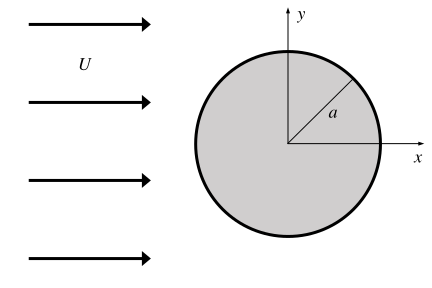
\includegraphics[width=0.7\linewidth]{Figures/Chapter3/fig_cyl_setup}
\caption{Fluid flows past the cylinder along the $x$-direction.}
\label{fig_cyl_setup}
\end{figure}

The other assumption we'll make is that the flow is irrotational.  This seems like a leap to make, though, since we don't even know what the flow \emph{is} yet.  But remember the vorticity equation (\ref{eq_vorticity}) -- for a steady two dimensional flow, the vorticity is conserved along streamlines.  Since the vorticity at infinity, where the flow is \emph{uniform}, is definitely zero, and every streamlines starts and ends at infinity, it follows that the flow is everywhere irrotational.

Wait, is our flow \emph{steady}?  Yes, as long as we examine the problem from the point of view of the flow already happening for a while; it's reached a steady state.  In practice, it doesn't take long for the fluid to do this.

To find the fluid velocity around the cylinder, we'll solve Laplace's equation.  It makes sense to use cylindrical coordinates here, given the symmetry of the boundary.  In cylindrical coordinates, then, Laplace's equation is
\begin{equation}
\label{eq_laplace_cyl}
\ddfdx{\phi}{r} + \frac{1}{r} \dfdx{\phi}{r} + \frac{1}{r^2} \ddfdx{\phi}{\theta} + \ddfdx{\phi}{z} = 0.
\end{equation}
Now, this is an example of two dimensional flow, so the $z$ term we can safely ignore.

Our boundary conditions are straightforward to write down.  First, at $r \to \infty$, we should have the uniform flow given by equation (\ref{eq_uniform}); we found the potential corresponding to this flow in Example \ref{ex_uniform}:
\begin{equation}
\label{eq_cyl_bc1}
\phi = Ur \cos \theta \quad  \text{as} \quad r \to \infty.
\end{equation}
Secondly, at $r=a$, we have the actual boundary.  Unlike viscous flows, ideal fluids must ``slip'' along a boundary; in this case, that means we must have the fluid velocity at $r=a$ be purely in the $\hat{\theta}$ direction.  In other words, we need $u_r = 0$; in terms of the potential (using the gradient in cylindrical coordinates), that's
\begin{equation}
\label{eq_cyl_bc2}
\dfdx{\phi}{r} = 0 \quad \text{at} \quad r=a.
\end{equation}

We'll solve Laplace's equation using separation of variables.  Let
\[
\phi(r, \theta) = R(r) \Theta(\theta).
\]
Then equation (\ref{eq_laplace_cyl}) becomes
\[
\Theta \frac{d^2R}{dr^2} + \frac{\Theta}{r} \frac{dR}{dr} + \frac{R}{r^2} \frac{d^2 \Theta}{d\theta^2} = 0,
\]
or, dividing by $R\Theta$ and multiplying by $r^2$,
\begin{equation}
\label{eq_cyl_sep}
\frac{r^2}{R} \frac{d^2R}{dr^2} + \frac{r}{R} \frac{dR}{dr} = -\frac{1}{\Theta} \frac{d^2 \Theta}{d \theta^2}.
\end{equation}
The left hand side of the equation is a function of $r$ only, while the right hand side is a function of $\theta$ only; they must therefore both be equal to a constant.  We'll call the this separation constant $k^2$.  The $\theta$ equation is then
\[
\frac{d^2 \Theta}{d\theta^2} = -k^2 \Theta,
\]
which has the solution
\[
\Theta (\theta) = A \sin k\theta + B \cos k\theta.
\]

We can apply our first boundary condition, equation (\ref{eq_cyl_bc1}), right away to eliminate the sine term, since we need only a cosine dependence as $r \to \infty$.  Comparing the form of equation (\ref{eq_cyl_bc1}) with our solution, we furthermore must have $k=1$.  Thus 
\begin{equation}
\Theta(\theta) = B \cos \theta.
\end{equation}

The radial part of equation (\ref{eq_cyl_sep}) (with $k = 1$) now reads
\[
r^2 \frac{d^2R}{dr^2} + r \frac{dR}{dr} - R = 0.
\]
We can solve this by trying a power-law solution of the form $R(r) = r^m$; it turns out that the general solution is
\[
R(r) = Cr + \frac{D}{r}.
\]
But our second boundary condition, equation (\ref{eq_cyl_bc2}), was that the first derivative of the potential goes to zero at $r=a$.  That means
\[
\frac{dR}{dr} = \left( C - \frac{D}{r^2} \right)_{r=a} = 0,
\]
and so $D = a^2 C$.

Combining the radial and angular equations gives us
\[
\phi(r, \theta) = R(r) \Theta(\theta) = F \left( r+\frac{a^2}{r} \right) \cos \theta,
\]
where $F=CB$ is our last remaining constant.  One more comparison with our boundary condition, equation (\ref{eq_cyl_bc1}), tells us that $F = U$.  So our solution to Laplace's equation is, finally, 
\begin{equation}
\phi(r, \theta) = U \left( r+\frac{a^2}{r} \right) \cos \theta.
\end{equation}

That's the potential; what about the fluid velocity?  No problem:
\[
\uu = \grad \phi,
\]
so
\begin{equation}
u_r(r, \theta) = U \left( 1 - \frac{a^2}{r^2} \right) \cos \theta
\end{equation}
and
\begin{equation}
u_\theta(r, \theta) = -U \left( 1 + \frac{a^2}{r^2} \right) \sin \theta.
\end{equation}
From $\uu$, we can sketch streamlines, which are shown in Figure \ref{fig_cyl_streamlines}.

\begin{figure}
\centering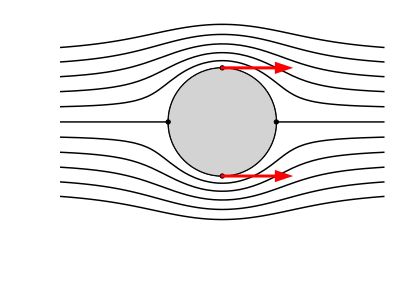
\includegraphics[width=0.7\linewidth]{Figures/Chapter3/fig_cylinder_stream}
\caption{The streamlines for the flow around the cylinder.  Note that there are stagnation points upstream and downstream of the cylinder ($\theta = 0$ and $\theta = \pi$), and the fluid has greatest velocity at the top and bottom ($\theta = \pi2$ and $\theta = 3\pi/2$).  \href{https://nbviewer.jupyter.org/github/josephmacmillan/IntroFluidDynamics/blob/master/Jupyter/3-IdealFluids.ipynb\#Figure-3.5:-Streamlines-for-flow-past-a-cylinder}{[Link to code]}}
\label{fig_cyl_streamlines}
\end{figure}

Let's examine the flow in a little more detail.  Note that, as necessary, $u_r=0$ at $r=a$.  On the boundary, the flow is purely angular, with speed 
\[
u_\theta = -2U \sin \theta \quad \text{at} \quad r=a.
\]
At $\theta = 0$ and $\theta = \pi$, then $u_\theta = 0$ and there is a stagnation point there (see Figure \ref{fig_cyl_streamlines}).  There is a maximum speed at $\theta = \pi/2$ and $\theta = 3\pi/2$ of
\[
u_{\theta, \text{max}} = 2U \quad \text{at} \quad r=a.
\]

What about the pressure in the fluid?  Well, we could apply Euler's equation to find it, but Bernoulli's principle provides a shortcut.  Since the flow is irrotational, $\grad H = 0$ and $H = p/\rho + \tfrac{1}{2} \uu^2 + gz = $ constant everywhere in the fluid.  In our analysis, though, we'll neglect the gravity term; we're only looking at the $(r, \theta)$ dependence of the pressure here, and gravity will only impose an overall vertical pressure gradient.

Let's first evaluate $H$ at infinity, where $\uu = (U,0,0)$ and we'll label the pressure $p_\infty$.  Then
\[
H = \frac{p_\infty}{\rho} + \tfrac{1}{2} U^2.
\]
Elsewhere in the fluid, it's
\[
H = \frac{p(r, \theta)}{\rho} + \tfrac{1}{2} \uu^2,
\]
where
\[
\uu^2 = \uu \cdot \uu = u_r^2 + u_\theta^2 = U^2 \left( 1 + \frac{a^4}{r^4} - 2\frac{a^2}{r^2} \cos 2\theta \right)
\]
(that last step required some algebra to clean up, though).  Since $H$ is constant, we have
\[
\frac{p(r, \theta)}{\rho} + \tfrac{1}{2} U^2 \left( 1 + \frac{a^4}{r^4} - 2\frac{a^2}{r^2} \cos 2\theta \right) = \frac{p_\infty}{\rho} + \tfrac{1}{2} U^2.
\]
Rearranging gives the pressure,
\begin{equation}
p(r, \theta) = p_\infty + \tfrac{1}{2} \rho \frac{a^2}{r^2} U^2 \left( 2 \cos 2\theta - \frac{a^2}{r^2} \right).
\end{equation}
Figure \ref{fig_cyl_pressure} shows the pressure around the cylinder; there is a region of high pressure at $\theta = 0$ and $\theta = \pi$, with low pressure at $\theta = \pi/2$ and $\theta = 3\pi/2$.  Not surprisingly, this is opposite the fluid velocity -- expected, since Bernoulli's theorem holds here.

\begin{figure}[t]
\centering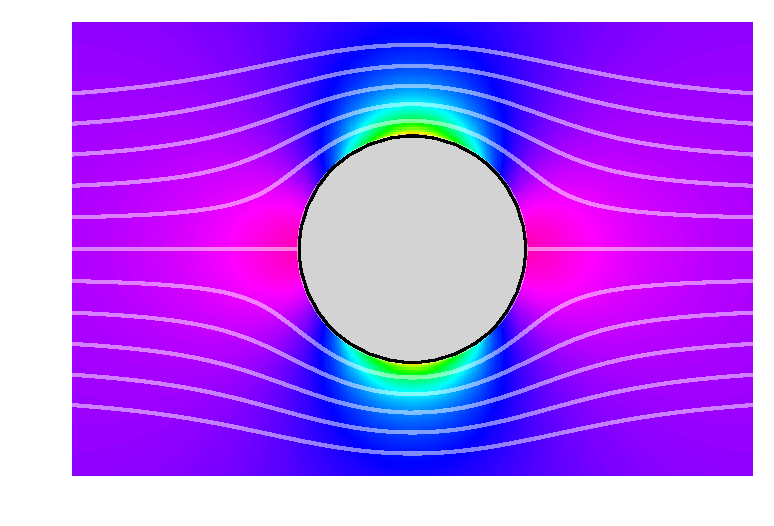
\includegraphics[width=0.8\linewidth]{Figures/Chapter3/fig_cylinder_pressure}
\caption{The pressure field of fluid flowing past a cylinder.  The pinkish regions are areas of high pressure, while the yellow/green areas are low pressure.  The streamlines are shown as well. \href{https://nbviewer.jupyter.org/github/josephmacmillan/IntroFluidDynamics/blob/master/Jupyter/3-IdealFluids.ipynb\#Figure-3.6:-Pressure}{[Link to code]}}
\label{fig_cyl_pressure}
\end{figure}








\section*{Problems}
\addcontentsline{toc}{section}{Problems}

\begin{problem}[Yet more vector calculus]
\label{prob_vc3}
Show that, for any vector field $\mathbf{v}$, you can write
\[
(\mathbf{v} \cdot \grad ) \mathbf{v} = (\curl \mathbf{v}) \times \mathbf{v} + \grad(\tfrac{1}{2} \mathbf{v}^2).
\]
\end{problem}

\begin{problem}[Please, no more vector calculus]
\label{prob_vc4}
Show that, for any two vector fields $\mathbf{F}$ and $\mathbf{G}$, you can write
\[
\curl (\mathbf{F} \times \mathbf{G}) = (\mathbf{G} \cdot \grad) \mathbf{F} - (\mathbf{F} \cdot \grad) \mathbf{G} + \mathbf{F} (\div \mathbf{G}) - \mathbf{G} (\div \mathbf{F})
\]
\end{problem}


\begin{problem}[The Rankine Vortex as a Model for Hurricanes]
A Rankine vortex is defined by the flow (in cylindrical coordinates)
\[
\mathbf{u}  = \left\{
 \begin{array}{l l}
    \Omega r \, \hat{\theta} & \quad \text{if $r < a$}\\
   \frac{\Omega a^2}{r} \, \hat{\theta} & \quad \text{if $r>a$,}
  \end{array} \right.
\]
where $\Omega$ and $a$ are constants (related to the wind speed and size of the ``core,'' respectively).  It serves as a useful model for a number of weather and atmospheric conditions, such as hurricanes, mesocyclones, and tornadoes.  

(a) Plot the wind speed as a function of distance, and calculate and plot the vorticity.

(b) To decide whether it is a useful model for hurricanes, I've provided (online) azimuthal wind speed data and vorticity data for Hurricane Katrina, which devastated New Orleans and the surrounding area in 2005.  The wind speed data has the first column as distance $r$ (in km) and the second column as azimuthal wind speed $u_\theta$ (in m/s).  The vorticity data has the first column as distance $r$ (in km) and the second column as vorticity $\omega$ (in $10^{-4}$ s$^{-1}$).

Use the Rankine vortex (RV) to model this hurricane; what values of $\Omega$ and $a$ give you the best fit?  Does the RV model the vorticity with those parameters as well?  Can you make any conclusions about how well the model does (e.g., is it better in some regions versus others?)

(c) Calculate the pressure throughout the hurricane and find the difference in pressure between r = 0 (the eye of the hurricane) and $r \to \infty$ (outside the storm).

(d) Finally, calculate the shape of the free surface (i.e., where the pressure is atmospheric). Plot the surface as a 3D surface. Compare this with photos of Katrina -- how does it look?
\end{problem}



\begin{problem}[The force on a cylinder]
We've already calculated the pressure in the fluid around a cylinder in Section \ref{sec_cylinder}, so it's a short leap to find the total force exerted on the cylinder by the fluid.

Consider Figure \ref{fig_cylinder_force}:  the force (per unit length of the cylinder) on a small angular section of size $a \, d\theta$ is
\[
d\textbf{F} = - p \hat{n}.
\]
Using this, show the total force on the cylinder is zero.  This is called \emph{D'Alembert's paradox} -- there's no drag on the cylinder, despite very obvious physical evidence to the contrary.  Does it make sense that the fluid exerts no force at all on the cylinder as it flows past?  Discuss this a bit.

\begin{figure}[t]
\centering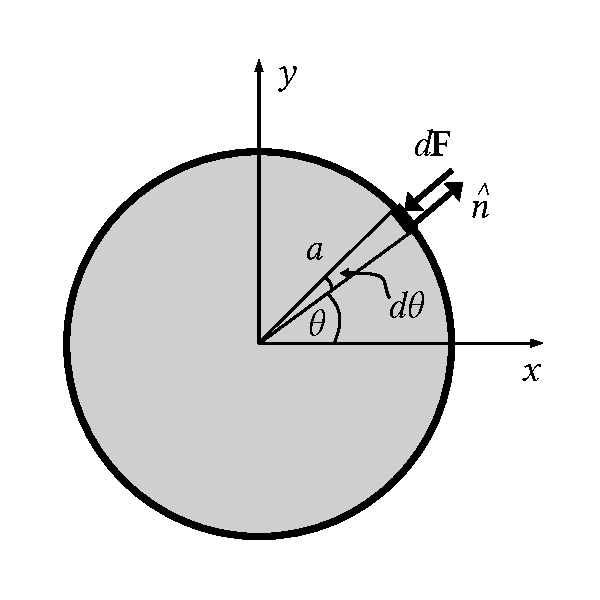
\includegraphics[width=0.5\linewidth]{Figures/Chapter3/fig_cyl_force}
\caption{The force on a small angular section of the cylinder.  The force is opposite the normal vector $\hat{n}$.}
\label{fig_cylinder_force}
\end{figure}

\end{problem}



\end{document}
